
\chapter{Implementation}

This chapter presents the implementation details of the proposed solution, including the initial architecture created, the process of finding and modifying a suitable malware, and the explanation of the final implementation.

\section{Creating the Implementation Environment} \label{sec:prerequisites}
Before starting the implementation, a secure environment was essential, as this thesis deals with malware. To achieve this, Oracle VM VirtualBox Manager, an open source virtualisation solution~\cite{website:oracleVirtualBox}, was installed to create three virtual machines. These included a leader machine and two other VMs called VM1 and VM2. While the leader machine is used to run all the server components, the other two are intended to mimic the IoT devices. Ubuntu was chosen as the operating system as it is the most widely used operating system for constrained devices as described in Section \ref{sec:hardSoftware}. This OS had to be changed later which will be described in Section \ref{section:IssuesOfInitialPrototype}. Since the hardware details can be customized later, no further thoughts were given to this at this stage. 

Ideally, a different machine than the main computer would be used to run all the virtual machines, but unfortunately this was not an option. However, to ensure the highest level of security for the machine and the network, several security measures were taken. All the machines created were put into an internal network. This is an option within VirtualBox that creates a software-based internal network where only the machines in the network can communicate with each other. In this way, the machines cannot communicate with the host machine or the outside world, which was exactly the aim as this prevents uncontrolled spreading. A side effect was that it was not possible to download anything from the Internet. 

The solution to this problem was a shared folder that could be accessed by the host computer and the virtual machines. For additional security, the shared clipboard has been disabled and the host machine has been placed on a guest network so that there are no other devices in the same network. Therefore, even in the unlikely case of the host machine being infected, the malware could not spread across the network except to the router. However, as the default password has been changed and the latest updates are automatically installed on the router, the risk of infection is negligible. Other security measures that were already in place included a different OS on my host computer and Malwarebytes anti-virus protection. Thus, the environment created was as secure as it could be. The described environment can be seen in Figure \ref{graphic:architecture}.


\begin{figure}[h!]
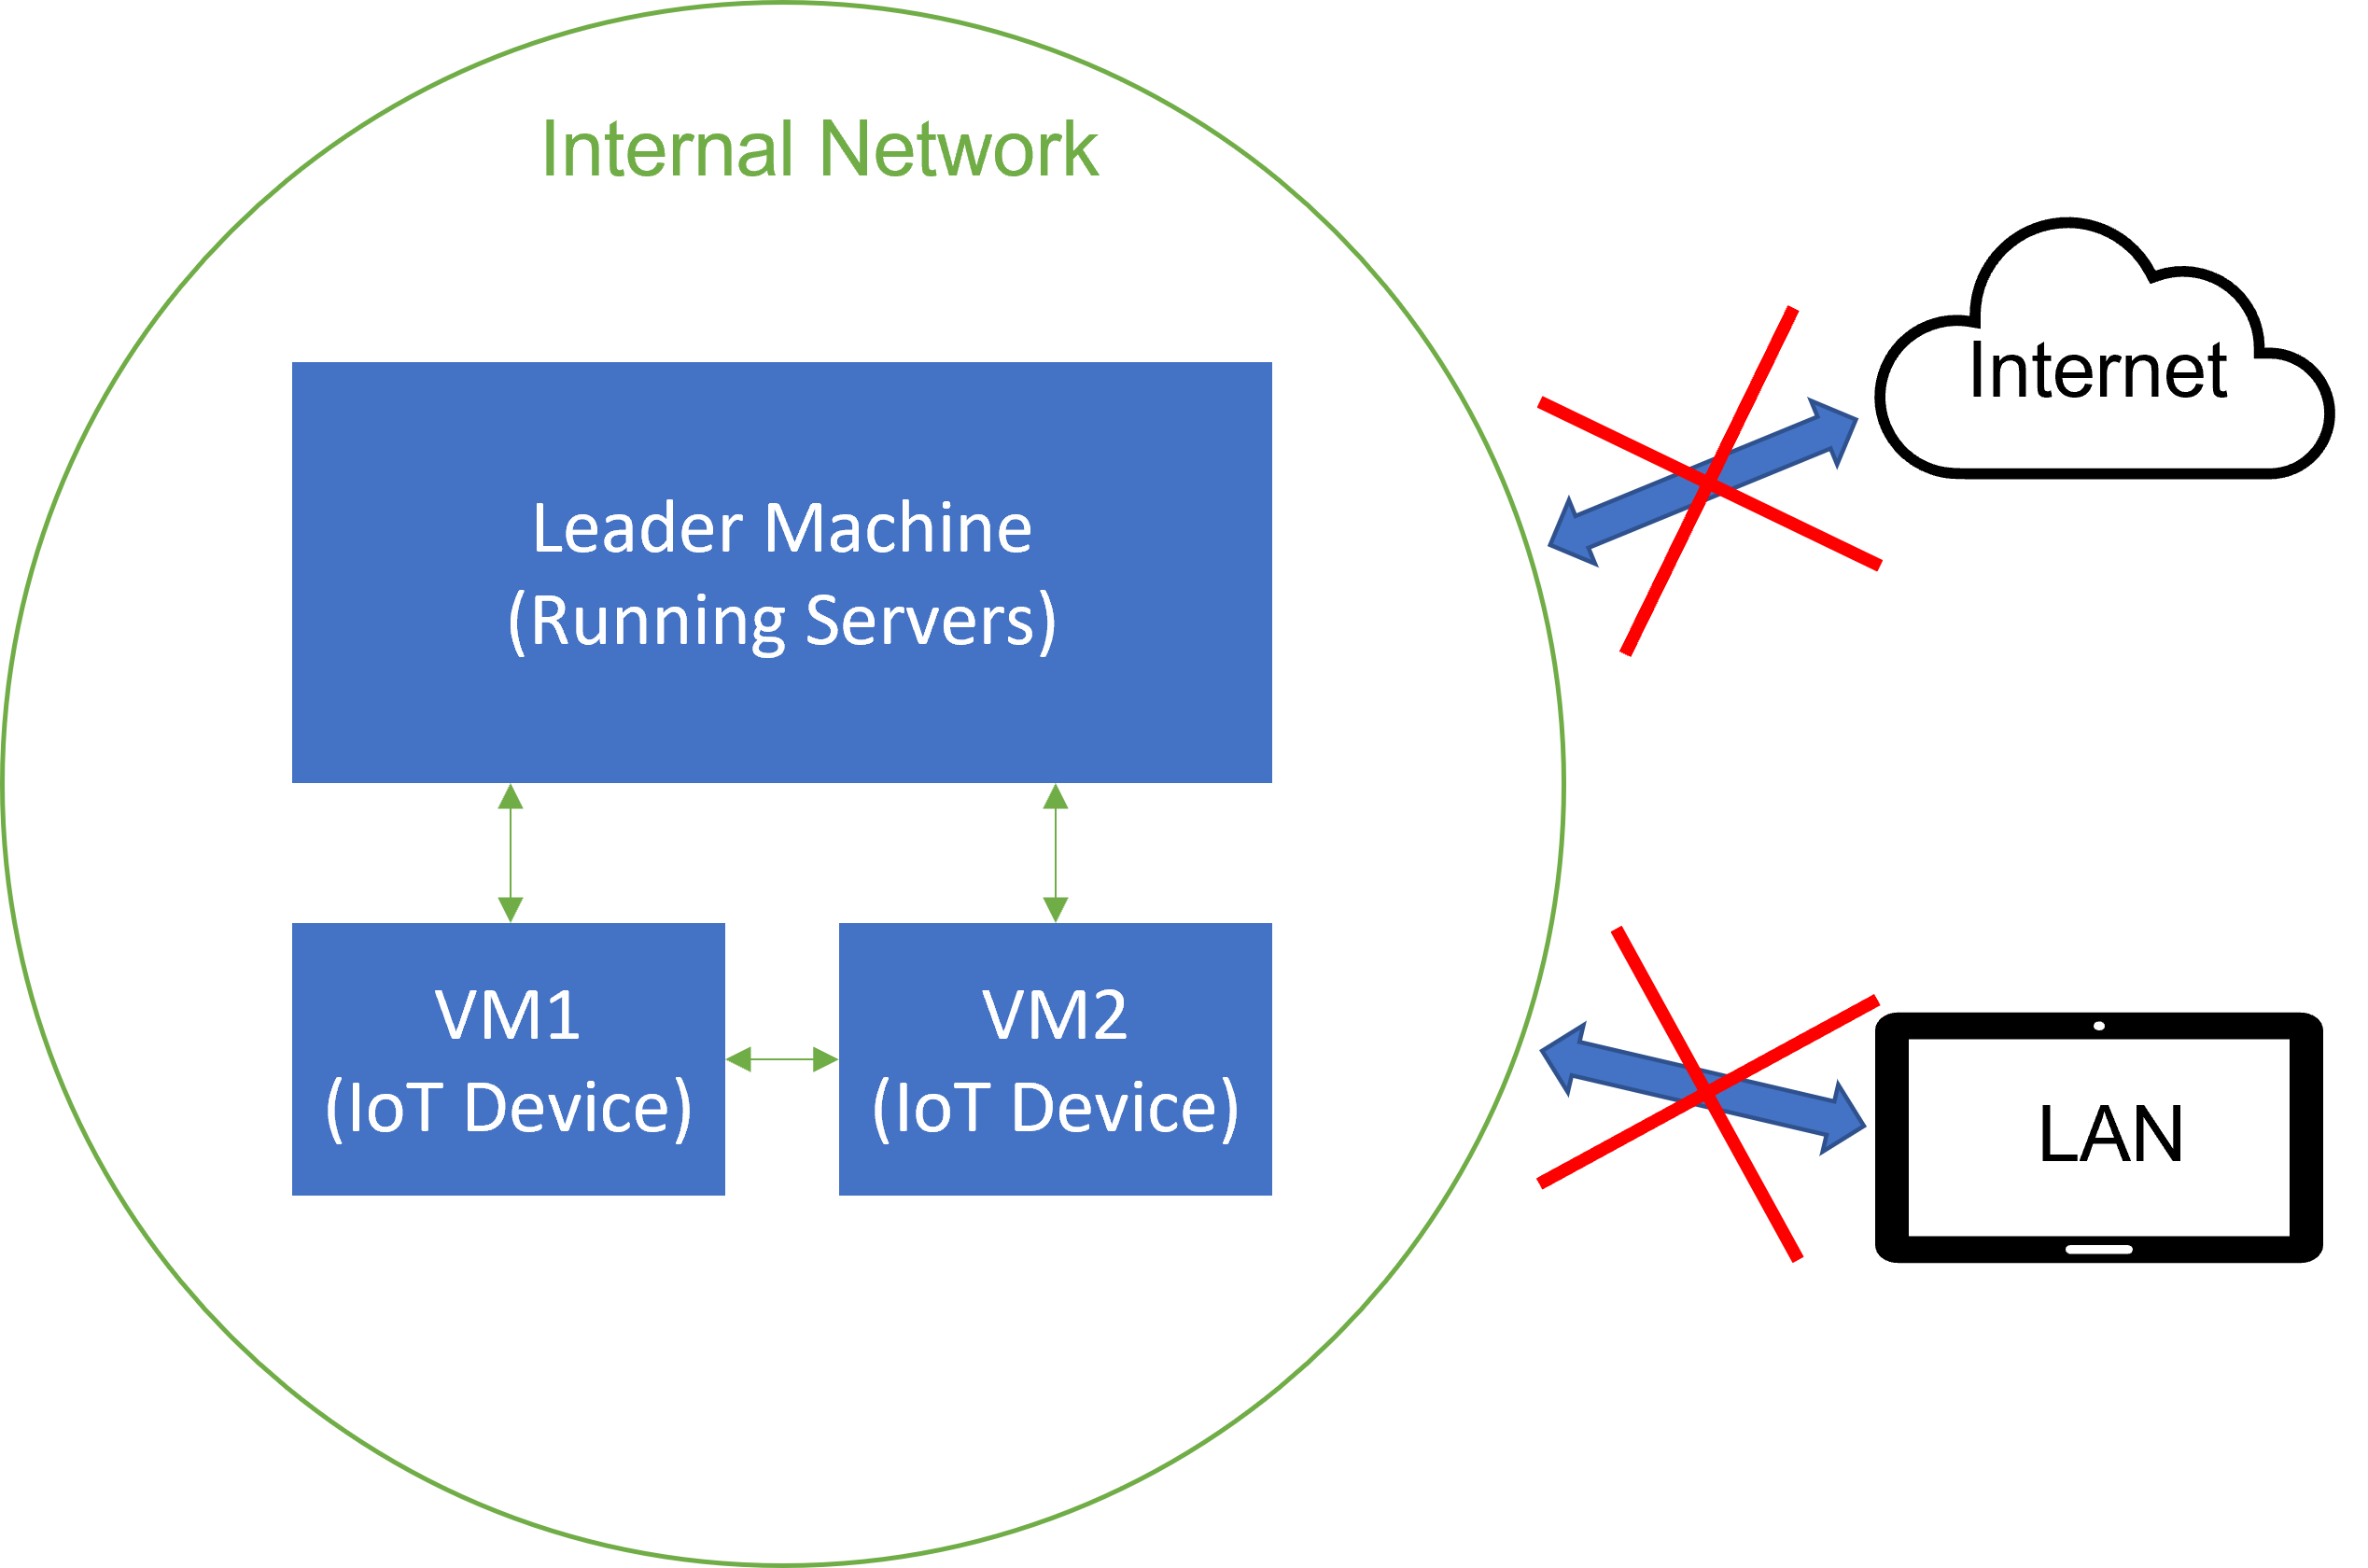
\includegraphics[scale=0.7]{assets/architecture.png}
\centering
\caption{The Created Environment With 3 Different VMs in an Internal Network Which Prevents the Malware From Spreading to Other Machines. }
    \label{graphic:architecture}
\end{figure}




\section{Initial Prototype} \label{section:initialPrototype}
The first prototype should help to better understand MTD from an implementation perspective, which should ultimately help to find appropriate solutions for the problem at hand. The architecture of this prototype was very similar to~\cite{article:Cedeno}. An overview of this architecture can be seen in Figure \ref{graphic:firstArchitecture}. The leader machine runs two applications, the \textit{MTD Deployer Client} and the \textit{MTD Deployer Server}. These two do not necessarily have to run on the same machine, but it is possible. The idea was to have these two programs do as much of the work as possible, given the hardware limitations of the IoT devices, at a later stage. The architecture is explained using the numbers in Figure \ref{graphic:firstArchitecture}.
\begin{enumerate}
    \item VM1 and VM2 continuously send information to the \textit{MTD Deployer Client}. This information consists of RAM usage and CPU usage. 
    \item The \textit{Deployer Client} continuously checks for anomalies in the information sent by VM1 and VM2. For simplicity, this anomaly is a RAM or CPU usage greater than 50\% in the last ten steps of the information sent.
    \item The \textit{Deployer Client} notifies the \textit{Deployer Server} of conspicuous behaviour in VM1 and VM2. 
    \item The \textit{MTD Deployer Server} then initiates the MTD techniques, which in this case is simply changing the private IP addresses of the virtual machines. The \textit{Deployer Server} uses the \textit{nmap} command to find all the occupied IP addresses in the network and sends each machine a new, unused IP address. 
    \item The VMs listen for commands sent by the \textit{Deployer Server} and then migrate to the newly sent IP address using the \textit{ifconfig} command. 
\end{enumerate}

\begin{figure}[tph]
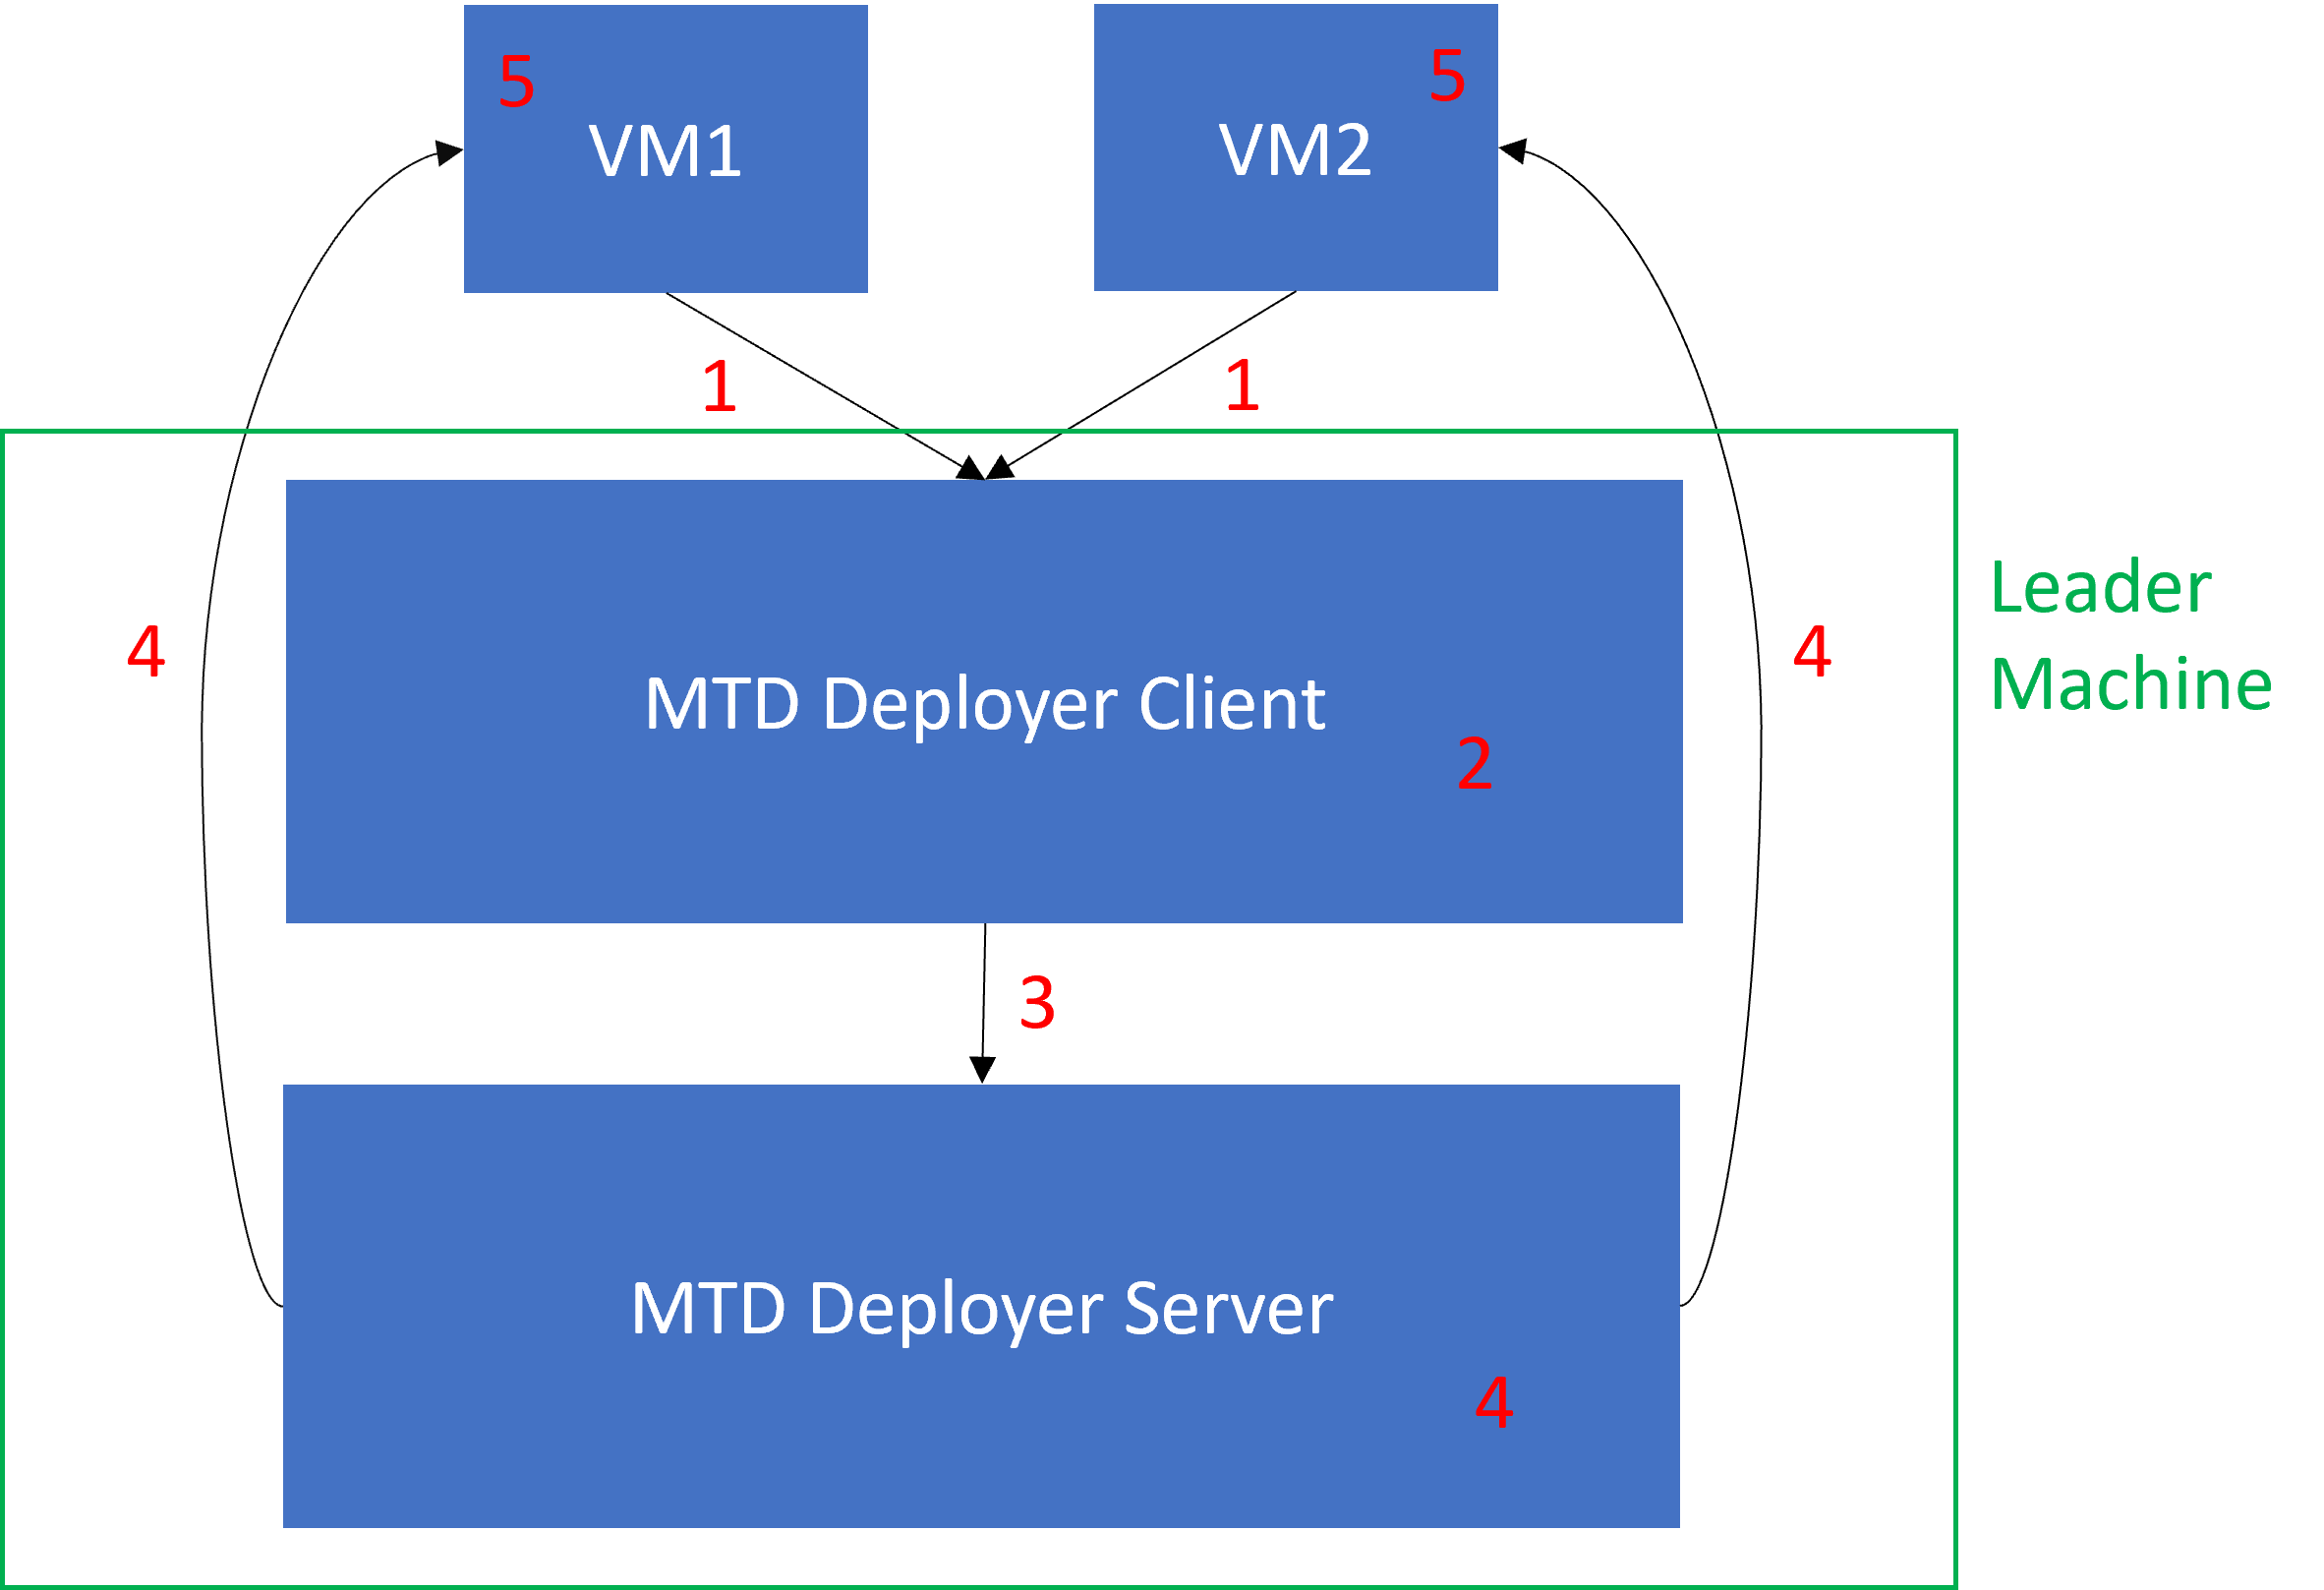
\includegraphics[scale=0.8]{assets/firstArchitecture.png}
\centering
\caption{The Architecture of the First Prototype.}
    \label{graphic:firstArchitecture}
\end{figure}

The cooperative part of this prototype is that if one VM detects malware, all VMs should initiate countermeasures, not just the affected one. This approach had several weaknesses, such as the VMs not checking that the migration to the IP address was working. This and other weaknesses were addressed in later implementations. 

This prototype was implemented in Python using sockets, which can be used to send messages across a network~\cite{website:realPythonSockets}. The prototype was also briefly tested by running all the Python scripts and manually setting the CPU usage of a VM to 100\%, whereupon the system handled the fake malware call. The \textit{Deployer Server} successfully sent messages to the VMs, which then changed their IP addresses according to the content of the messages. Thus, everything worked as expected and it was possible to continue. 


\section{Finding Malware Samples} \label{main:bashlite}
The first goal after the initial prototype was to find a suitable malware for this thesis. This was necessary for a number of reasons: Firstly, the malware had to be studied to see how it interacts with the system in order to develop the most appropriate countermeasures. This included studying the underlying code where possible. Second, it would be more meaningful to evaluate the MTD techniques with real malware. However, finding suitable malware proved to be a difficult and extremely time-consuming task. On the one hand, this was due to the rarity of malware code on platforms such as GitHub, which is understandable, as otherwise anyone could easily compile and distribute the malware. On the other hand, there were a number of requirements that the malware had to meet:
\begin{itemize}
    \item The malware should ideally target IoT devices. Although it would have been possible to use malware targeting desktop devices, the aim was to use IoT malware to get as close to the real world as possible.
    \item The malware code should ideally be openly available for study and modification. This was important as the malware will likely need to be tailored to work for this thesis. It was also important to study the code in order to find possible weaknesses in the malware.
    \item The malware had to run on the created VMs in order to execute and play with it. This was ultimately to help understand and test the weaknesses of the malware. 
    \item The malware must have a spreading functionality. This is necessary because the goal of this thesis is to use a cooperative MTD mechanism to mitigate/prevent the spreading of the malware.  
\end{itemize}

Especially the last point proved to be difficult in the end. Several code repositories such as GitHub and malware repositories such as MalwareBazaar were searched, but no suitable malware could be found. On GitHub, there exists a repository~\cite{website:iot-malware-2017} that contains the code of several IoT malware, such as Bashlite, Mirai, Lightaidra and some others. However, all of them had problems (incomplete, no spreading functionality, not executable) or were too complex to work with, as they might need to be slightly rewritten. There were other repositories, such as~\cite{website:githubMirai}, which again provided the Mirai code, or~\cite{website:githubBashlite}, which provided the same code as the first repository. The problem with MalwareBazaar was that it provided mostly executables, which was unsuitable, since code to read and modify was an essential requirement. Finally, Bashlite was chosen, even though it was initially not executable and lacked an important piece of code.

\section{Bashlite}
This section presents various aspects of Bashlite. These include the changes required to get Bashlite running, explanations of how the malware works, and an analysis of where possible MTD techniques could be applied. Note that from now on the term "client" will be used to refer to the machines that act as infected and susceptible IoT devices. This is not to be confused with the \textit{MTD Deployer Client} that runs on the leader machine and is part of the MTD framework.


The starting point was the code from~\cite{website:githubBashlite}, even though every Bashlite on Github seemed to provide the same code. Bashlite consists of two files, a server file and a client file, both written in C. Having encountered the C programming language only once in a university course and never used it again, the C language was the first obstacle, especially as the Bashlite code contained few explanatory comments. Once the general idea of the code was clear, the goal was to run it on the created VMs to see if this would work. The C files were compiled using the GNU compiler collection, which contains compilers and development tools~\cite{website:gccincredicuild} and was pre-installed on the Ubuntu systems.

Unfortunately, the execution completely failed in the case of the client script. The \textit{server.c} file was executable on the leader machine, but the client threw a fork error that was unknown to me until then. \textit{Fork} is used to create a child process, whereupon the parent and child process use separate memory spaces~\cite{website:fork}. Although several possible solutions, such as running it with \textit{sudo} or checking that the system had not reached its maximum number of processes were tried, the problem remained. After some time and a lot of trial and error, the idea came up that the underlying operating system might be the problem and not the script itself. 

Thus, new machines were set up, but this time with the Raspberry Pi Desktop OS~\cite{website:raspberryOSDesktop}. As shown in Section \ref{graphic:IoTOSs}, the Raspberry Pi OS (formerly Raspbian) had the second-largest share of all Linux distributions in IoT devices, so it is a suitable alternative. After everything was set up, the client was immediately executable on the Raspberry Pi OS. Therefore, it is not clear whether the OS was the problem in the first place, but changing it was one possible solution. Below follows a description of Bashlite's server and client and how the two files were modified for this thesis. 

\subsection{Bashlite Server}
The Bashlite server basically opens two ports on the executing machine. The first port (8888) was already defined in the code and is the port to which a "management" connects. This management then controls the server and the clients. So, to broadcast to the clients and do anything in general, one must first telnet to port 8888 of the server machine and enter a password, otherwise the server will not do anything useful with the clients. The other port opened by the server is passed as an argument when the script is started, along with the number of threads to create. The port used in this thesis was 6667, but this does not matter as long as the port is free; all that matters is that the same port is included in the client code, as this is the port to which the clients will connect after infection. The bridge between the management and the client is the broadcast function. This function takes the strings sent by the management and broadcasts them to all the clients, which then execute some commands/functions based on those strings. The important thing to note here is that no plain Bash commands can be sent directly from the management to the clients, so sending an "ls" as the management will not cause the clients to do anything. The server automatically broadcasts a "PING" to all clients every 60 seconds. Figure \ref{graphic:controlStreamServer} shows the basic control flow of the server. 

\begin{figure}[tph]
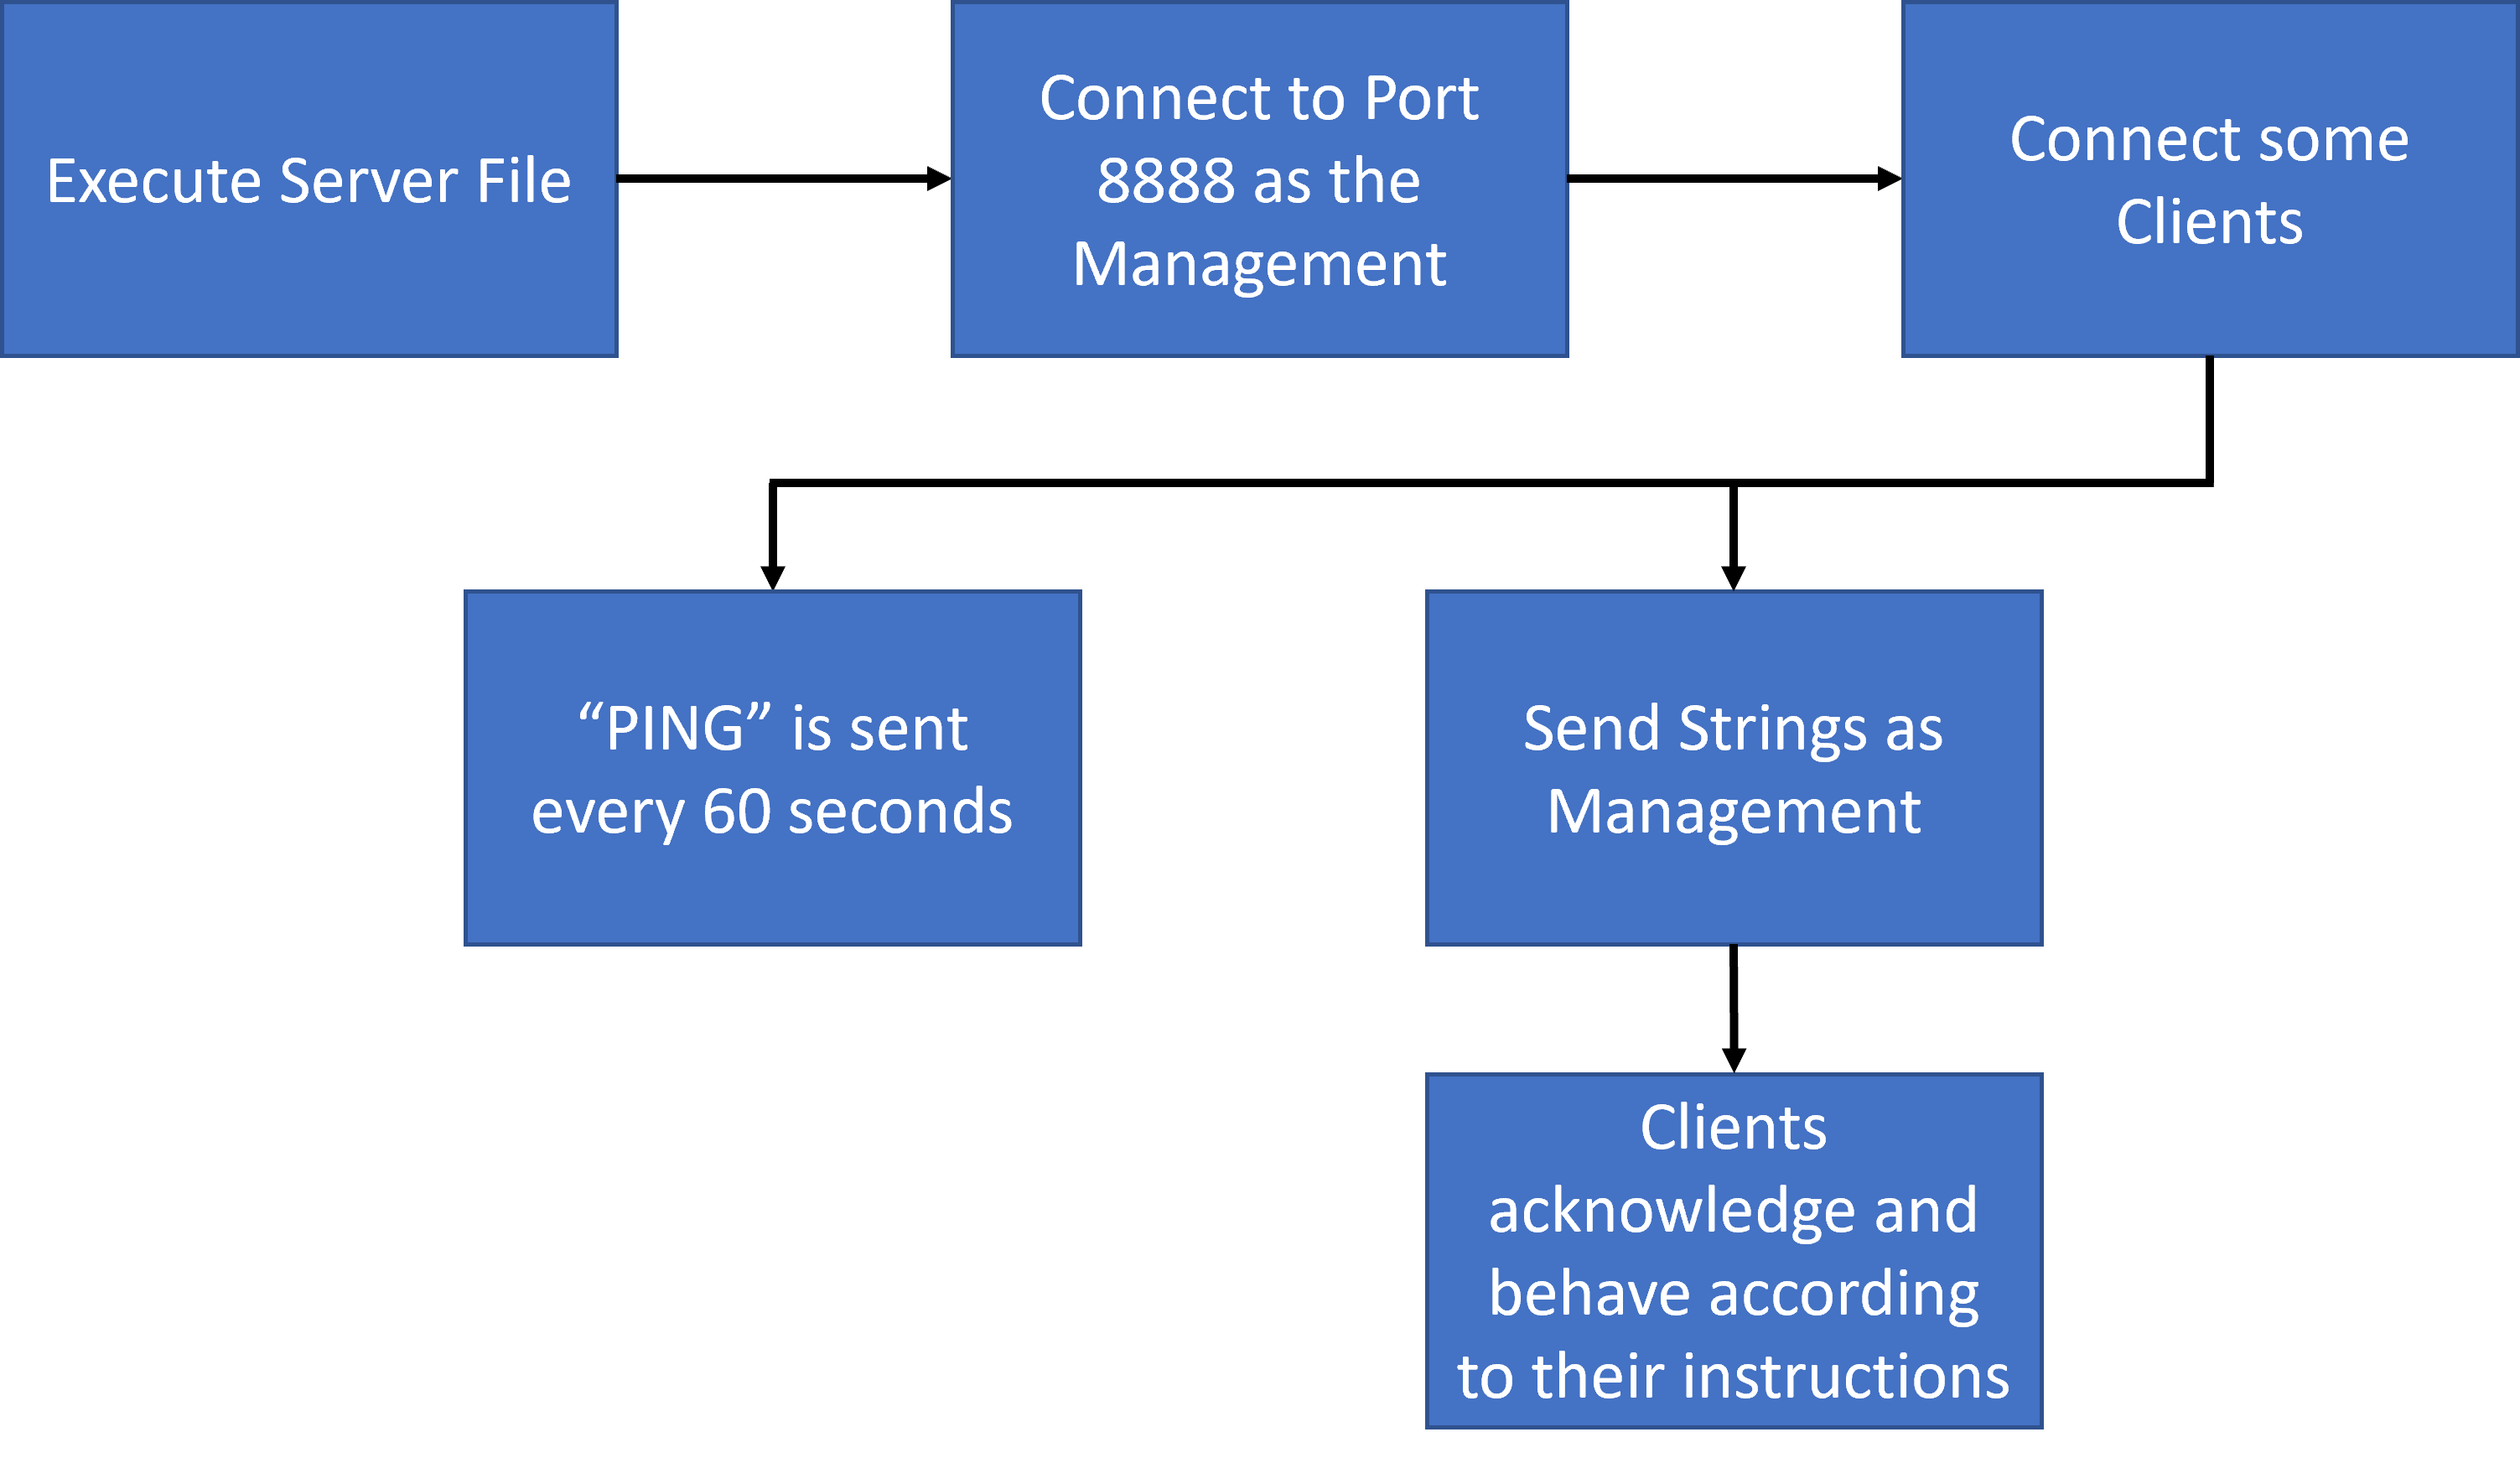
\includegraphics[scale=0.6]{assets/controlStream.png}
\centering
\caption{A Simplified Control Flow of the Server File of Bashlite.}
    \label{graphic:controlStreamServer}
\end{figure}

\subsection{Bashlite Client}
The client is much more complex than the server and contains many more lines of code. At the beginning of the client file, the IP address of the command server must be specified, and two \textit{char} arrays containing default usernames and passwords are created. Later in the code, these are used to check whether another device found is not properly secured, and if so, the correct username and password combination is stored.
Various helper functions follow (e.g. various printing options, or a function that searches for a string in the buffer), but these are not important for a rough understanding of the general concept. 

One important helper function is \textit{getRandomPublicIP()}. This function first generates a random IP address using the \textit{rand()} function, and then has a while block that basically checks if the IP address is public, and otherwise generates a new IP that is checked again, and so on. An invalid example would be if the first two octet portions of the IP address were 192.168.x.x, as this is a range for private IP addresses. Ultimately, the function returns a valid public IP address.

There are two other essential functions in the client, the \textit{processCmd()} function and the \textit{StartTheLelz()} function. The former processes strings sent by the management. The function waits for strings, whereupon the client returns a string or starts the execution of a function. Interestingly, some management strings are handled in this \textit{processCMD()} function (e.g. SCANNER commands) and some strings are handled directly in the client's \textit{main()} function (e.g. "DUP"). Some commands have to start with an exclamation mark, otherwise they would not be recognized by the client. Useful inputs were
\begin{itemize}
    \item "DUP", which terminates all client sessions
\item "!SCANNER ON" and "!SCANNER OFF", which starts and stops the \textit{StartTheLelz()} function.
    \item "!SH" \textit{arguments} which can be used to run shell commands on the clients. 
\end{itemize}

The \textit{StartTheLelz()} function is the most important and also the most complex function of the client. At the beginning of this function a struct called \textit{telstate\_t} is created. This struct contains several attributes such as an IP address, the state, the username index or the password index and is inserted into a file descriptor array (fds[]). The state attribute is essential as there are 12 different cases in this function and the state attribute determines which case the current file descriptor is in. The function starts with case 0 and then increments to the next case if all requirements in the current case are met. The following paragraph briefly describes the main tasks of each case. 

Case 0 checks if it is theoretically possible to connect to an IP returned by \textit{getRandomPublicIP()}, and also increments the index of the username and password if the current file descriptor was sent back by Case 3 or 5. Case 1 checks for timeouts and the like. Case 2 checks if a login is requested by the connected IP address, Case 3 sends the username and also resets the file descriptor to Case 0 if the username was wrong, otherwise it sets the state to 4. Case 4 checks if a password is requested, Case 5 sends the current password of the file descriptor, and Case 6 checks if the password is correct and resets the file descriptor to Case 0 if not. Case 7 checks if the shell is accessible and Case 8 checks if Busybox is installed. Case 9 either sends a report to the server or continues with the subsequent cases which were not needed. The simple report sent to the server is just a string in the format "REPORT IPaddress:username:password". 
Figure \ref{graphic:flowChartClient} shows the process of the client in a simplified flowchart. 


\begin{figure}[tph]
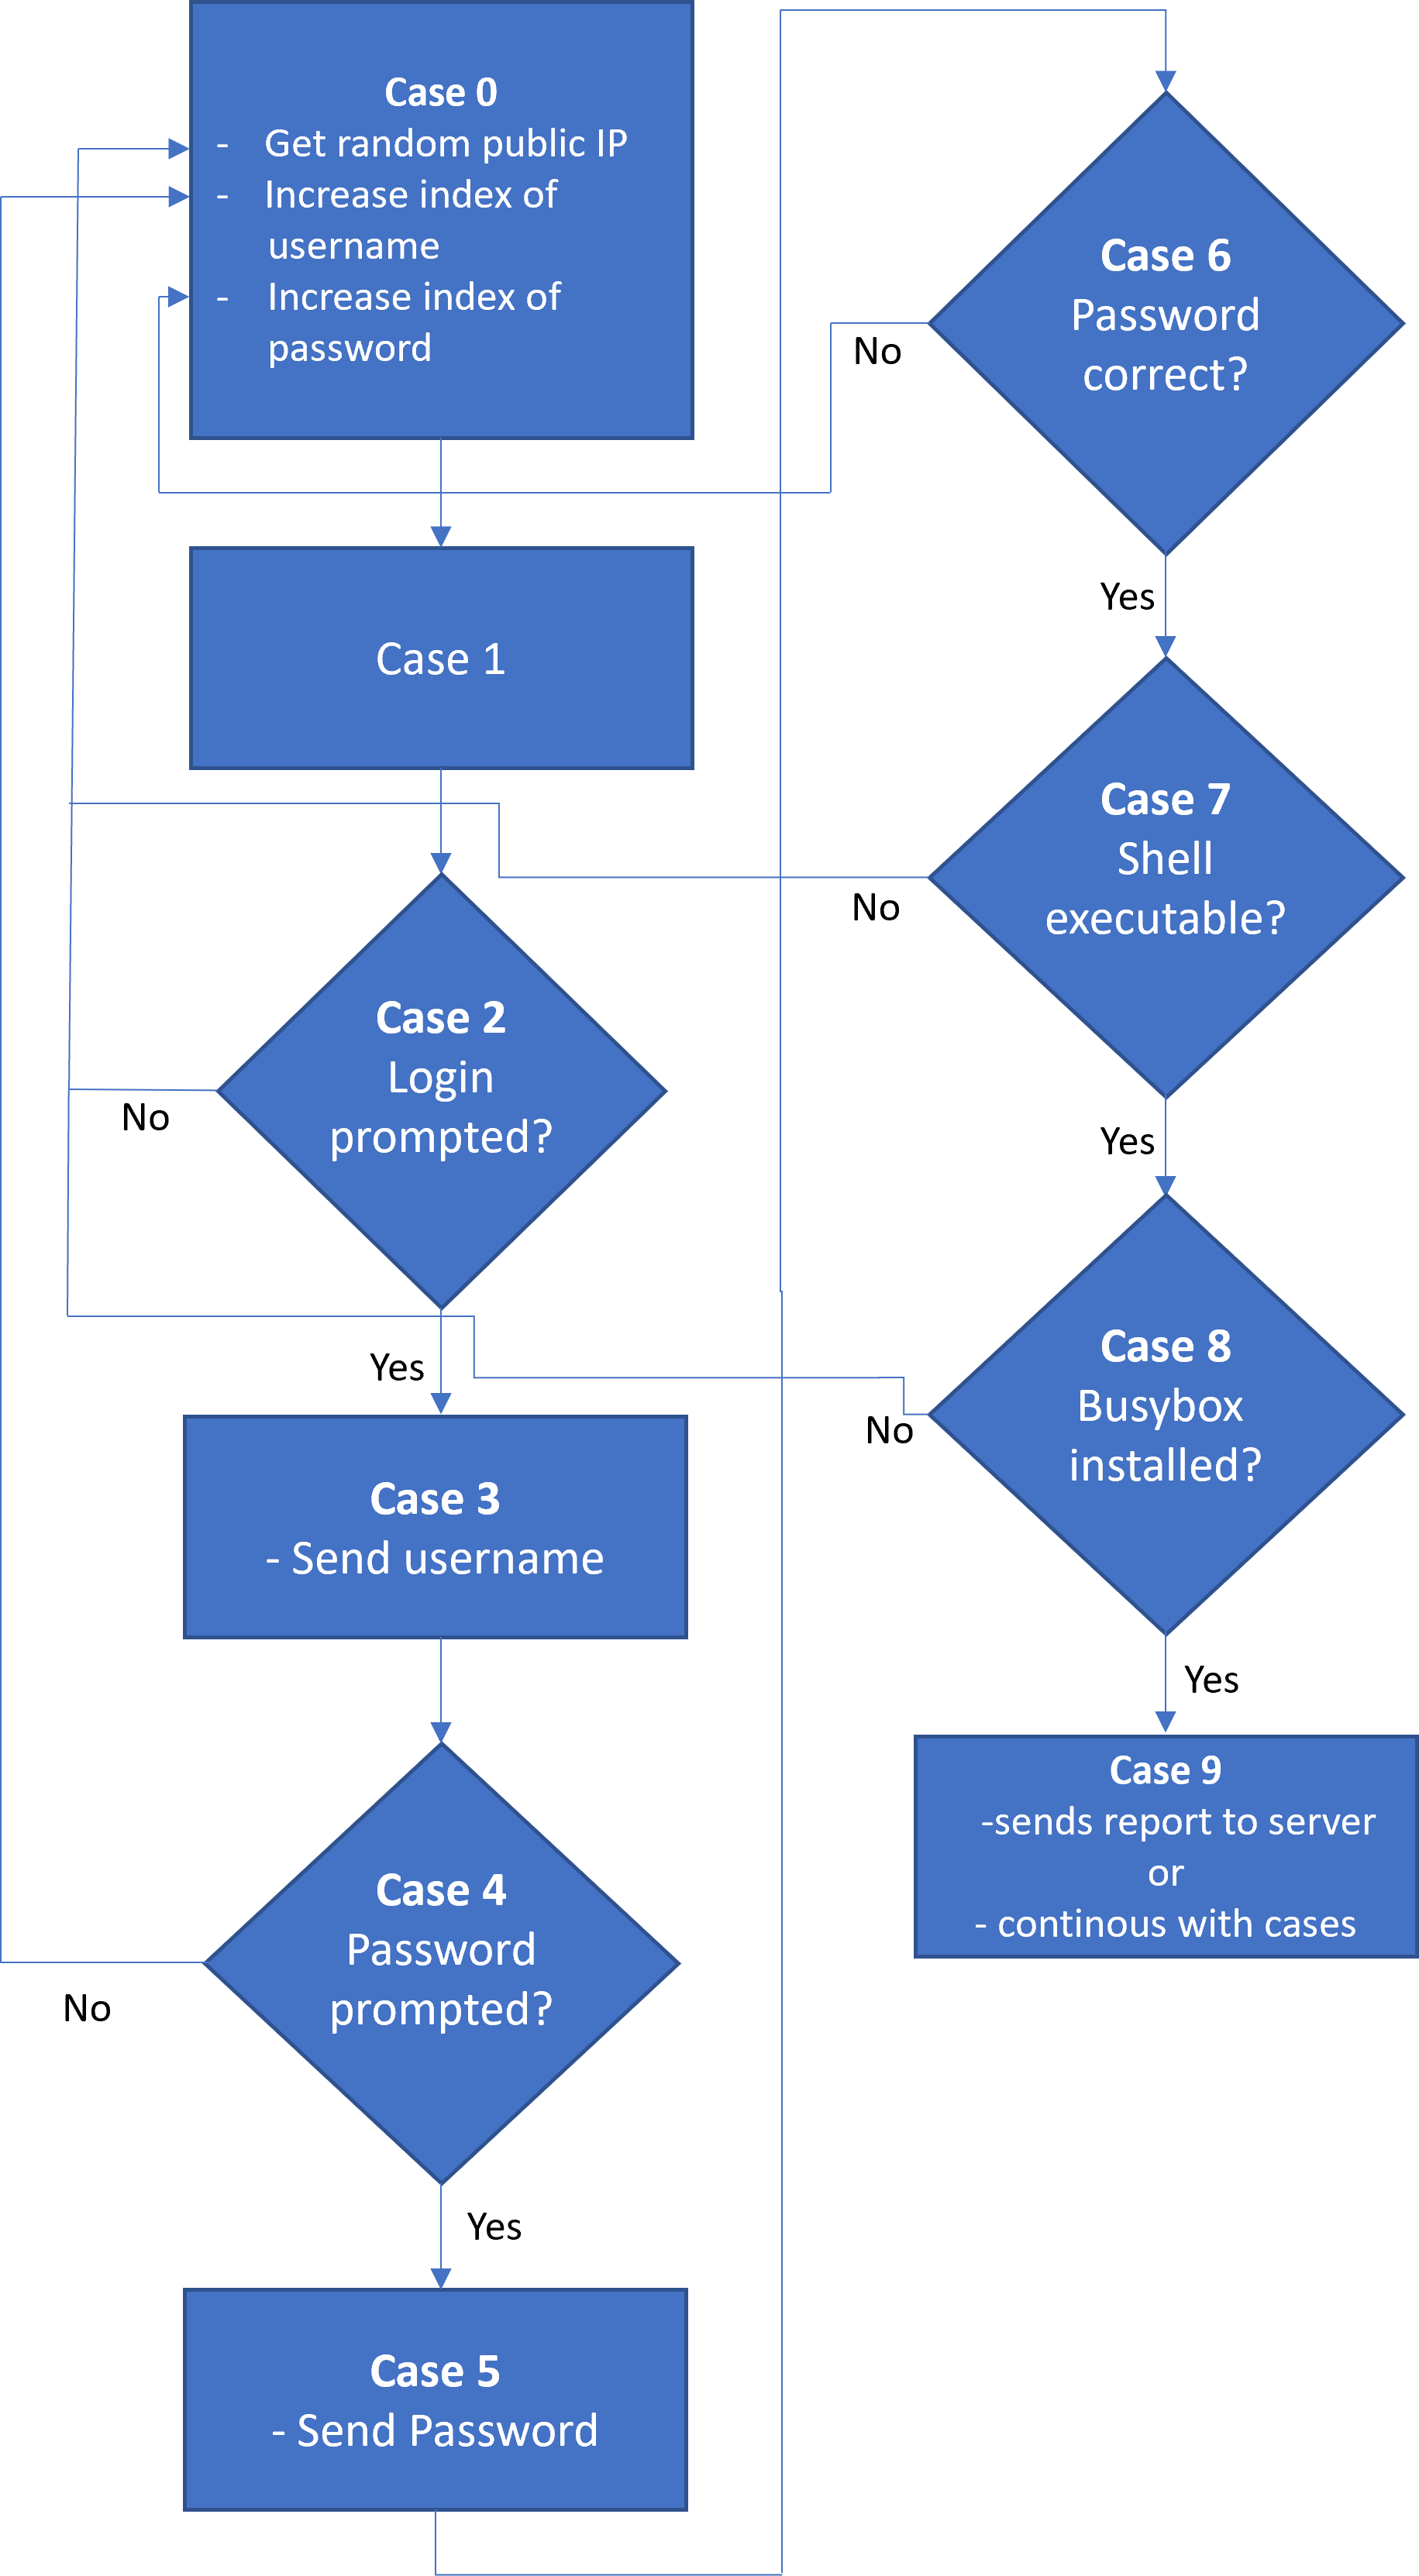
\includegraphics[scale=0.8]{assets/flowChartClient.png}
\centering
\caption{A Simplified Flow Chart of the Bashlite Client's Essential 	\textit{startTheLelz()} Function, Which Searches for Other Susceptible Devices. The Incoming Arrows to Case 0 Directly Point to the Action That Will be Executed.}
    \label{graphic:flowChartClient}
\end{figure}


\subsection{Code Modifications}
In order to get Bashlite to work as it is supposed to, several parts of the code had to be modified. This subsection describes those changes. The client was simpler to modify, probably because the code was intended to run as it was from the start.
In addition to many print statements to make the code understandable, the first step was to adapt the IP address of the command server and the arrays of usernames and passwords. Since the username and password of the susceptible machine are known, the corresponding combination was put into these arrays and the rest was deleted. Additionally, the script initializes another variable called "stillRunLelz". This variable was necessary because when the scanner on the first machine resumed scanning after sending the report to the server, the server often had trouble recognising that a second machine was now connected. So a workaround was to run the outermost while loop of the \textit{startTheLelz()} function for as long as "stillRunLelz" was 1, and after another vulnerable machine was sent to the server, "stillRunLelz" was set to 0 and the scanner stopped. This would certainly not be an applicable solution in a real malware, but it was sufficient for this thesis, as one additional infected machine was enough to test the concept.

The \textit{getRandomPublicIP()} function was also modified to return the IP address of the susceptible machine directly. Again, this would not make sense in real malware, but it sped up the development process without compromising the quality. Another problem was that the code never got further than case 6. This was solved by investigating where it failed and then sending it directly to case 7. Case 9 also checked a condition that was somehow not met, but this was solved by ignoring the condition and simply sending the report to the server at the beginning of case 9. These were all changes that had to be made to get the client to work so that a report of the vulnerable machine was sent to the server.



The server was more complex to adapt because some of the code was missing. Again, the first step was to add print statements to get a deeper understanding of how the server works. The second step was to add the missing code. This involved code to automatically exploit the IP address with the information sent by the client's scanner. To develop this, a separate C file was created so that Bashlite would not have to be continuously restarted. The code in this new file splits the report string into substrings to separate the IP address, username and password. The C function \textit{strtok()} with ":" as delimiter helped to achieve this. The rest was more complex, as the server still had to automatically connect to the susceptible machine, copy the client file to that machine, and run the client file. The best way to do this was with a Bash script called from the \textit{server.c} file with the \textit{system} call. The first attempt of a Bash script using Telnet for the connection failed, probably due to the back and forth interaction between the two machines. The next attempt was an \textit{expect} script. These scripts talk to other programs, know what to expect from them and give them the corresponding response~\cite{website:linuxExpect}. 

The \textit{expect} script starts with a timeout command of 30 seconds, so that it would not run for too long if it somehow failed. After that, the script creates variables for the arguments that are passed when the script is called. The call must be made in the following way:

\[ \mbox{telnetConnection.except \textit{IPAddress} \textit{username} \textit{password} \textit{fileToSend}}  \]

The first three arguments are given by the report string, the last one was a convenience in case a different file was to be sent to the client. The next step was to spawn the telnet command with the \textit{IPAddress} argument, whereupon the script expected the string "raspberry login:" and then sent the \textit{username} argument. This pattern continued until the \textit{expect} script connected to the susceptible machine via Telnet. The script then needed to copy the client file from the server machine to the susceptible machine. This copying functionality was important because it could have provided another defence option at a later stage. Since installing additional packages or creating an ssh key or password was not an option, the options to transfer the file were limited. This brought \textit{netcat} into focus, as it provided a good way to transfer the client file~\cite{website:netcat}.

Thus, the susceptible machine should open a \textit{netcat} connection on a port and then wait for the server to send the file over that connection. This worked perfectly when typed directly into Bash from both the client and the server, but it became more complicated than anticipated in the \textit{expect} script due to two constraints. The first was that the client obviously had to open a connection before anything could be sent from the server, and the second was that it was somehow impossible to send the files from the \textit{expect} script on the local machine. 

There were considerations to take the sending of the files out of the \textit{expect} script (and have it done by another script), but this was not practical. The reason for this was that the \textit{expect} script would then have to run partially (until it opened the \textit{netcat} connection on the susceptible machine), then pause until the client file was sent by another script, and then continue running the rest of the \textit{expect} script. The solution to this problem was to swap the server and client \textit{netcat} tasks. Previously, the vulnerable machine would open a connection and wait for the file to be sent from the server machine. Now the server machine opens a port to send the corresponding file and waits for the susceptible machine to request it. This made it possible to first run the \textit{netcat} command on the server and then start the \textit{expect} script in the same \textit{system()} call in C as the \textit{expect} script requested the file from the server.
Additionally, the content of the client file had to be pipped into \textit{netcat} on the server side, otherwise the transfer would fail. The final command can be seen in Algorithm \ref{lst:Pseudocode openNetcatStartExpect.py}.
\\


\begin{lstlisting}[caption={The Bash Command Used to Open a Netcat Connection From the Server to Send the File Once the Client Requested it and to Start the \textit{Expect} Script},label={lst:Pseudocode openNetcatStartExpect.py}]
cat fileToSend | netcat -q 5 -l 9899 & expect telnetConnection.expect IPAddress username password
\end{lstlisting}

Algorithm \ref{expectPseudocode} shows the \textit{expect} script in pseudocode. Now everything worked and experiments with MTD techniques and malware spreading were possible.
\\

\begin{lstlisting}[caption={The \textit{Expect} Script in Pseudocode},label={expectPseudocode}]
SET timeout 30
SET IPaddress to argument 0
SET username to argument 1
SET password to argument 2
SET fileToSend to argument 3
CONNECT to IPaddress with telnet
EXPECT "raspberry login"
SEND username variable
EXPECT "password"
SEND password variable
SEND netcat command to request the file
SEND sleep for 7 seconds
SEND command to make the requested file executable
EXPECT "password for"
SEND password variable
SEND sleep for 3 seconds
SEND execute client file
EXIT expect script
\end{lstlisting}


\subsection{Analysis of Bashlite} \label{analysisOfBashlite}
This section presents an analysis of Bashlite. This includes possible levers where MTD techniques could be applied to mitigate Bashlite.

 
As part of the analysis of Bashlite, many timing properties had to be checked. This required selecting suitable hardware properties for the VMs as a first step. As described in Section \ref{sec:prerequisites}, the hardware details were not a concern initially. To simulate a Raspberry Pi device, hardware similar to that used by~\cite{article:vonderAssen} was used, consisting of a 1.5 GHz CPU and 3.7 GB of RAM. The device running the VMs is a Surface Book 1 with 16 GB of RAM and an Intel Core i7-6600U dual-core CPU running at between 2.60 GHz and 3.40 GHz~\cite{website:intelInfo}. In VirtualBox it is possible to specify how many cores a VM can use and also the execution cap for those cores. Unfortunately, it is not possible to simply give the VM a frequency for its processor (e.g. 1.5 GHz). Thus, the performance information provided by the Windwows task manager had to be used as a reference to calculate the required execution cap. The task manager indicated that the laptop's base speed is 2.81 GHz. This appeared to be correct on average (even with all VMs running). Thus, each infected VM was given one core and an execution cap of 53\%, because 53\% of 2.81 GHz is about 1.5 GHz. In addition, the virtual machines have 3.7 GB RAM allocated to them by VirtualBox.


An infection process of Bashlite can be divided into four different phases, which are presented below. 
\begin{enumerate}
\item The first phase is when the infected client scans for susceptible devices and sends the information to the Bashlite server.
\item The second phase is when the server receives the report from an infected device and initializes the Telnet connection to the susceptible client. The duration of this phase is extremely short.
\item The third phase begins as soon as the Telnet connection to a susceptible device is started.
\item The fourth phase begins when the Bashlite client is launched on the susceptible machine.
\end{enumerate}


The first important data to get was the number of seconds these Bashlite phases took to complete. It is important to note that this could be different for a more sophisticated/varied malware or much better hardware on the devices, but Bashlite could serve as a reference. To achieve this, Bashlite was run 10 times and the time was measured by hand. Due to the various scripts on the server side, it was too complex to measure the time programmatically, so it was faster to do it manually. Other reasons were that it was not necessary to know the exact times and that the phases always took about the same number of seconds. The only time a script measured the execution time was in phase 2, as this period is too short to measure by hand. For phase 1, all time values were between 14 and 17 seconds, with an average of 15.5 seconds. Phase 2 lasted an average of 0.00007 seconds, making it negligible. Phase 3 time values ranged from 60 to 63 seconds with an average of 62 seconds. Thus, on average, 62 seconds pass before the susceptible machine is infected. The long duration of phase 3 is due to the \textit{expect} script written to connect, fetch the client file from the Bashlite server and execute it. This \textit{expect} script needed several sleeps to complete the actions, and the Telnet connection also takes some time. Perhaps the whole script could be written differently, but this was not possible without putting too much effort in it. 
Figure \ref{graphic:timelinePhases} shows the corresponding timeline, where phase 2 and 3 have been combined and the phases are colour-coded according to whether or not it is still possible to mitigate the spreading to the second device. 


\begin{figure}[tph]
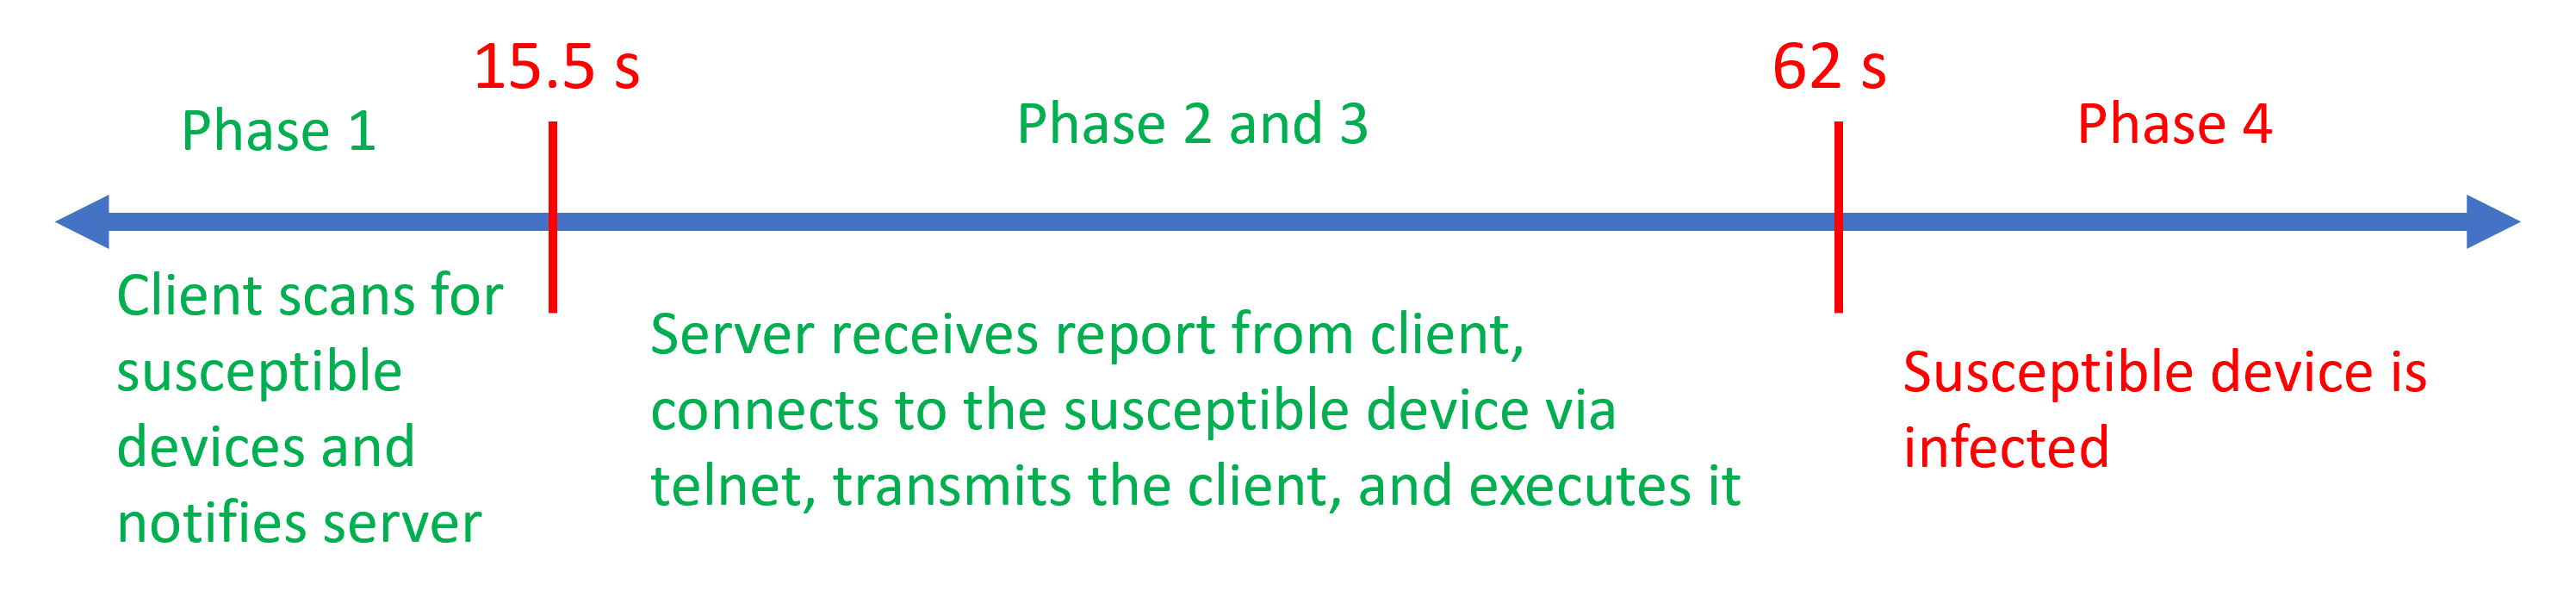
\includegraphics[scale=0.7]{assets/timelinePhases.png}
\centering
\caption{The Timeline Showing the Different Phases of a Bashlite Infection of one Susceptible Device.}
    \label{graphic:timelinePhases}
\end{figure}


%This allowed me to assess whether the proposed MTD techniques would also work against Mirai without running it. Even though there is a big difference in the code, it is obvious that Mirai's scanner also targets telnet ports, specifically port 23 and port 2323. The latter is often used as an alternative for port 23~\cite{website:gitSpeedGuide}. So it is safe to say that MTD techniques targeting these ports should work, at least in theory, for Mirai as well. The same holds for the "HEH" malware presented in Section \ref{subsection:P2PIoTBotnets}, as this malware also uses port 23 and port 2323 to infect devices~\cite{website:trendMicroUncleanable}. Even though I focus on Bashlite's characteristics below, MTD techniques that target ports 23 and 2323 should also be able to mitigate the spreading of Mirai and HEH. I will return to this in the evaluation. 
%\todo{see if the ip change also woud work for mirai}

%In addition to Bashlite, a part of the section deals with Mirai~\cite{website:githubMirai}. Even though Mirai is too complex to examine in detail in a short period of time, I compared Mirai's scanner file to the one of Bashlite to see, if they share the same weaknesses. 





%es chan jo au sii, dass de virus no anderi sache macht wie nur mitem command server verbindet, drum macht sinn wenn men scho vorher unterbindet

\section{Final Implementation} \label{section:finalImplementation}
This chapter presents the final implementation based on the analysis of Bashlite in Section \ref{analysisOfBashlite}. The implementation is based on the same structure in terms of VMs as the initial prototype in Section \ref{section:initialPrototype}. Again, the structure consists of three different virtual machines. The first is a leader machine running two applications, the \textit{MTD Deployer Client} and the \textit{MTD Deployer Server}. Both applications consist of two Python files, one of which acts as a listening socket, while the other contains the essential helper functions for the listening socket. For example, the \textit{MTD Deployer Server} has a listening Python file called \textit{listenToDeployerClient.py} and a \textit{sendToDevices.py} that sends the MTD execution commands to the devices.

The other two machines are the clients that mimic the IoT devices and also consist of two files each. The \textit{sendToDeployerClient.py} notifies the \textit{Deployer Client} when malware has been found, and the \textit{listenToDeployerServer.py} executes the corresponding MTD technique using the information sent by the \textit{sendToDevices.py}.
Even though this chapter briefly explains every file, the focus lies on \textit{sendToDevices.py} (\textit{Deployer Server}) and \textit{listenToDeployerServer.py} (client), as these two form the basis of the MTD techniques. However, before explaining the code, this section first introduces the chosen MTD techniques and how they relate to the background information from Section \ref{section:background}. 

\subsection{Implemented MTD Techniques} \label{section:implementedMTDTechniques}
The analysis of Bashlite described in Section \ref{analysisOfBashlite}, together with the working implementation of Bashlite described in Section \ref{main:bashlite}, provided the opportunity to search for suitable MTD techniques. These techniques should ideally protect against classic botnets and P2P IoT botnets. The first subsection below describes the implemented MTD techniques based on the analysis of Bashlite in Section \ref{analysisOfBashlite}, and the second subsection theoretically evaluates how these MTD techniques against Bashlite could protect against Mirai and HEH.


\subsubsection{Implemented MTD Techniques Based on the Analysis of Bashlite}
The first phase of Bashlite ends with the report sent from the infected client to the Bashlite server.~\cite{article:vonderAssen} and further experiments in this thesis have shown that it is possible to disrupt the connection between the Bashlite client and the Bashlite server by changing the IP address of the client. If the connection is disrupted before phase 2 begins, the report can be prevented from being sent, resulting in the best possible mitigation case. Once the second phase begins, the IP address change of the originally infected machine (VM1) will have no effect on the spreading of Bashlite to the susceptible machine (VM2). Of course, the IP address change should still be executed to disconnect the infected machine from the server, but this has no advantage in terms of spreading to the susceptible machine (VM2). This makes the second technique all the more important. The idea of this second technique is to move the Telnet port of the susceptible machines for some time while Bashlite is rendered harmless on the infected machine. This essentially hides the susceptible machines from the infected machine's scanner. 

This Telnet service port change technique works in phase 1. As just described, this prevents the infected machine's scanner from finding the susceptible machines. This technique theoretically also works in phase 2, although it is unlikely that the Telnet service port change is applied at this point because phase 2 is so short. The port change also works in phase 3, but it requires a small adjustment because once the connection between a susceptible machine and the Bashlite server is established, the port change has no effect. Thus, a potential Telnet connection must first be killed, and then the port changes must be applied to ensure that this susceptible machine is completely unreachable to a Bashlite scanner. In phase 4, the second machine is already infected, but the Telnet service port change should still be applied to all other machines in the network, as it could protect other, not yet infected machines (which were not present in the setup). Figure \ref{graphic:timeline} graphically shows the MTD techniques in combination with the phases. Note that the colours only indicate whether the applied MTD technique can prevent Bashlite from spreading to the susceptible machine. So a red font does not mean that the technique should not be applied, but that it has no effect on the Bashlite infection of other machines in the network. A green font means that the Bashlite spreading can be completely mitigated, a yellow font means that the spreading to the susceptible machine could not be mitigated, but the port change could still help other machines in the network. 

\begin{figure}[tph]
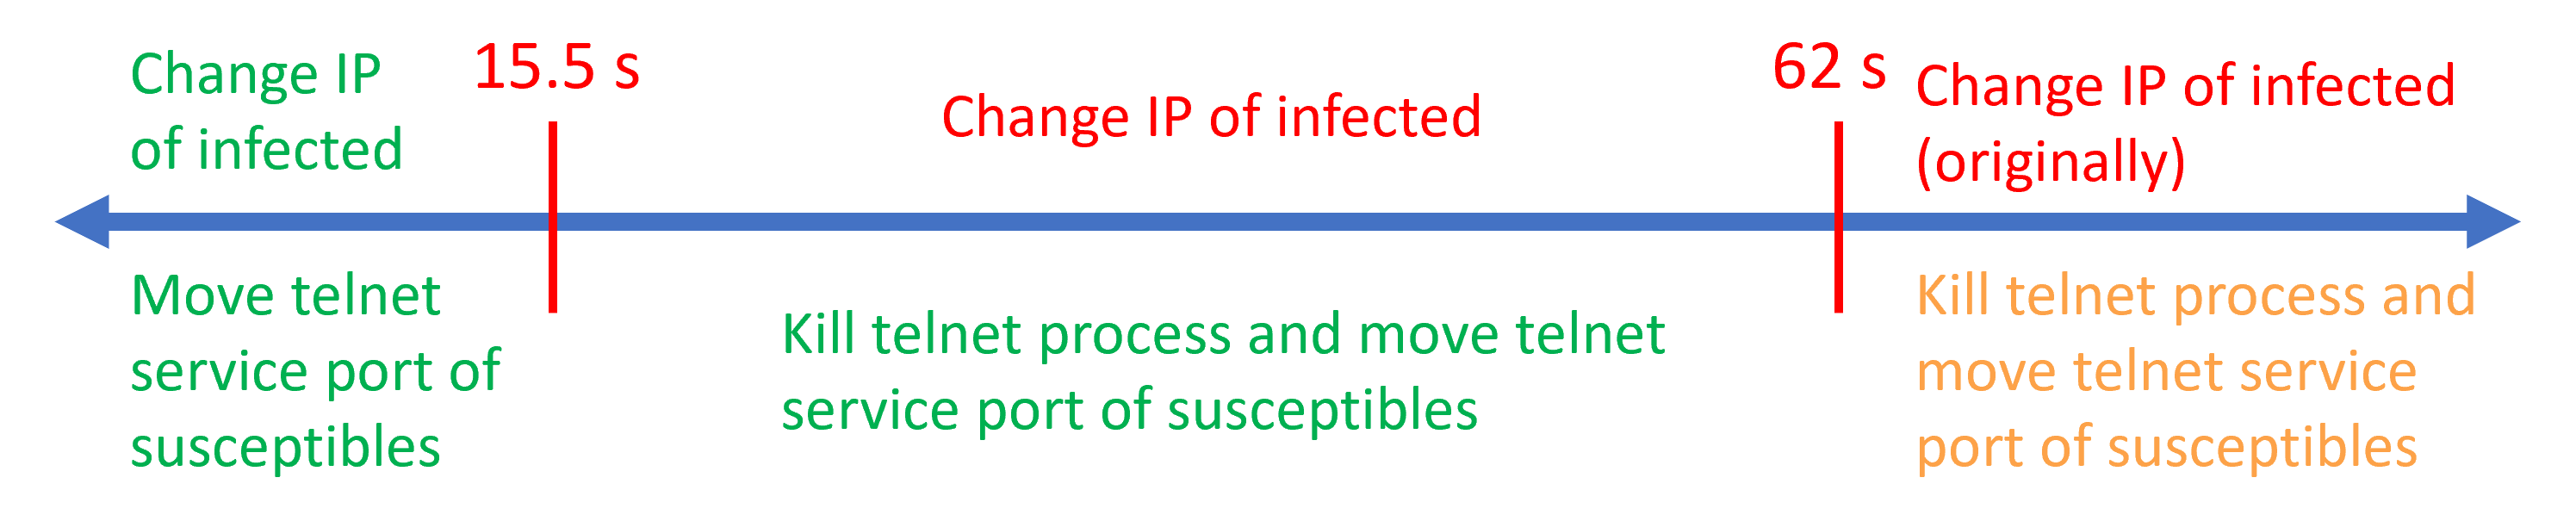
\includegraphics[scale=0.7]{assets/timeline.png}
\centering
\caption{The Timeline of an Infection With Bashlite of a Susceptible Device, Showing When the Mitigation is Still Possible.}
    \label{graphic:timeline}
\end{figure}

\subsubsection{Theoretical Evaluation of MTD Techniques Against Mirai and HEH}
A quick examination of Mirai's scanner file allowed an assessment of whether the proposed MTD techniques would work against Mirai without running it. Although there is a big difference in the code, it is obvious that Mirai's scanner also targets Telnet ports, specifically port 23 and port 2323. The latter is often used as an alternative for port 23~\cite{website:gitSpeedGuide}. The same holds for the HEH malware presented in Section \ref{subsection:P2PIoTBotnets}, as this malware also uses port 23 and port 2323 to infect devices~\cite{website:trendMicroUncleanable}. It is therefore safe to say that MTD techniques protecting port 23 (2323) should also work against Mirai and HEH, at least in theory. This is not the case for the IP address change. Although it is not possible to test it in the scope of this thesis, Mirai has a teardown functionality that is triggered when no response is received from the C\&C server. After this teardown, the client simply reconnects to the C\&C server, making the IP address change only a temporary obstacle. As for the HEH malware, it is not possible to predict the impact of the IP address change due to the unavailability of the code. However, as these types of botnets are extremely dangerous by nature, it is all the more important to prevent them from spreading. Changing the Telnet service port can therefore be considered an essential tool against all three malware types.

Once the required MTD techniques had been chosen, they needed to be defined according to the background information given in Section \ref{section:background}. This chapter introduced the three elements that define MTD techniques~\cite{article:Cai}. These three elements are "what", "how" and "when" and are used to formally describe the solution below. 

\subsubsection{Formal Definition of the Applied MTD Techniques}
The "what" to move is the IP address value and the port value of the Telnet service. The domain from which these two values are taken is defined in a configuration file, so that the user can choose in which range the value of the moving parameter should be. Of course, any IP address or port already occupied in the network or on the machine is automatically removed from this domain.  
The "how" is completely random. A random IP address or port value that is within the specified range but not yet in use will be used to replace the current moving parameter value. The final element is the "when" to move. As Bashlite has been shown to be detectable~\cite{article:vonderAssen}, the proposed solution uses an event-based decision process that includes a proactive and a reactive component. The IP address change technique is the reactive component, as it reacts to the detection of Bashlite and then initiates the countermeasures. In a sense, the port change is both reactive and proactive. Although it is also triggered by the detection of Bashlite (reactive), it also acts as a proactive component on the uninfected machines, as the technique attempts to get ahead of a Bashlite infection. The information just described can be seen graphically in Table \ref{graphic:tableAppliedMTDTechniques}.

\begin{table}[tph]
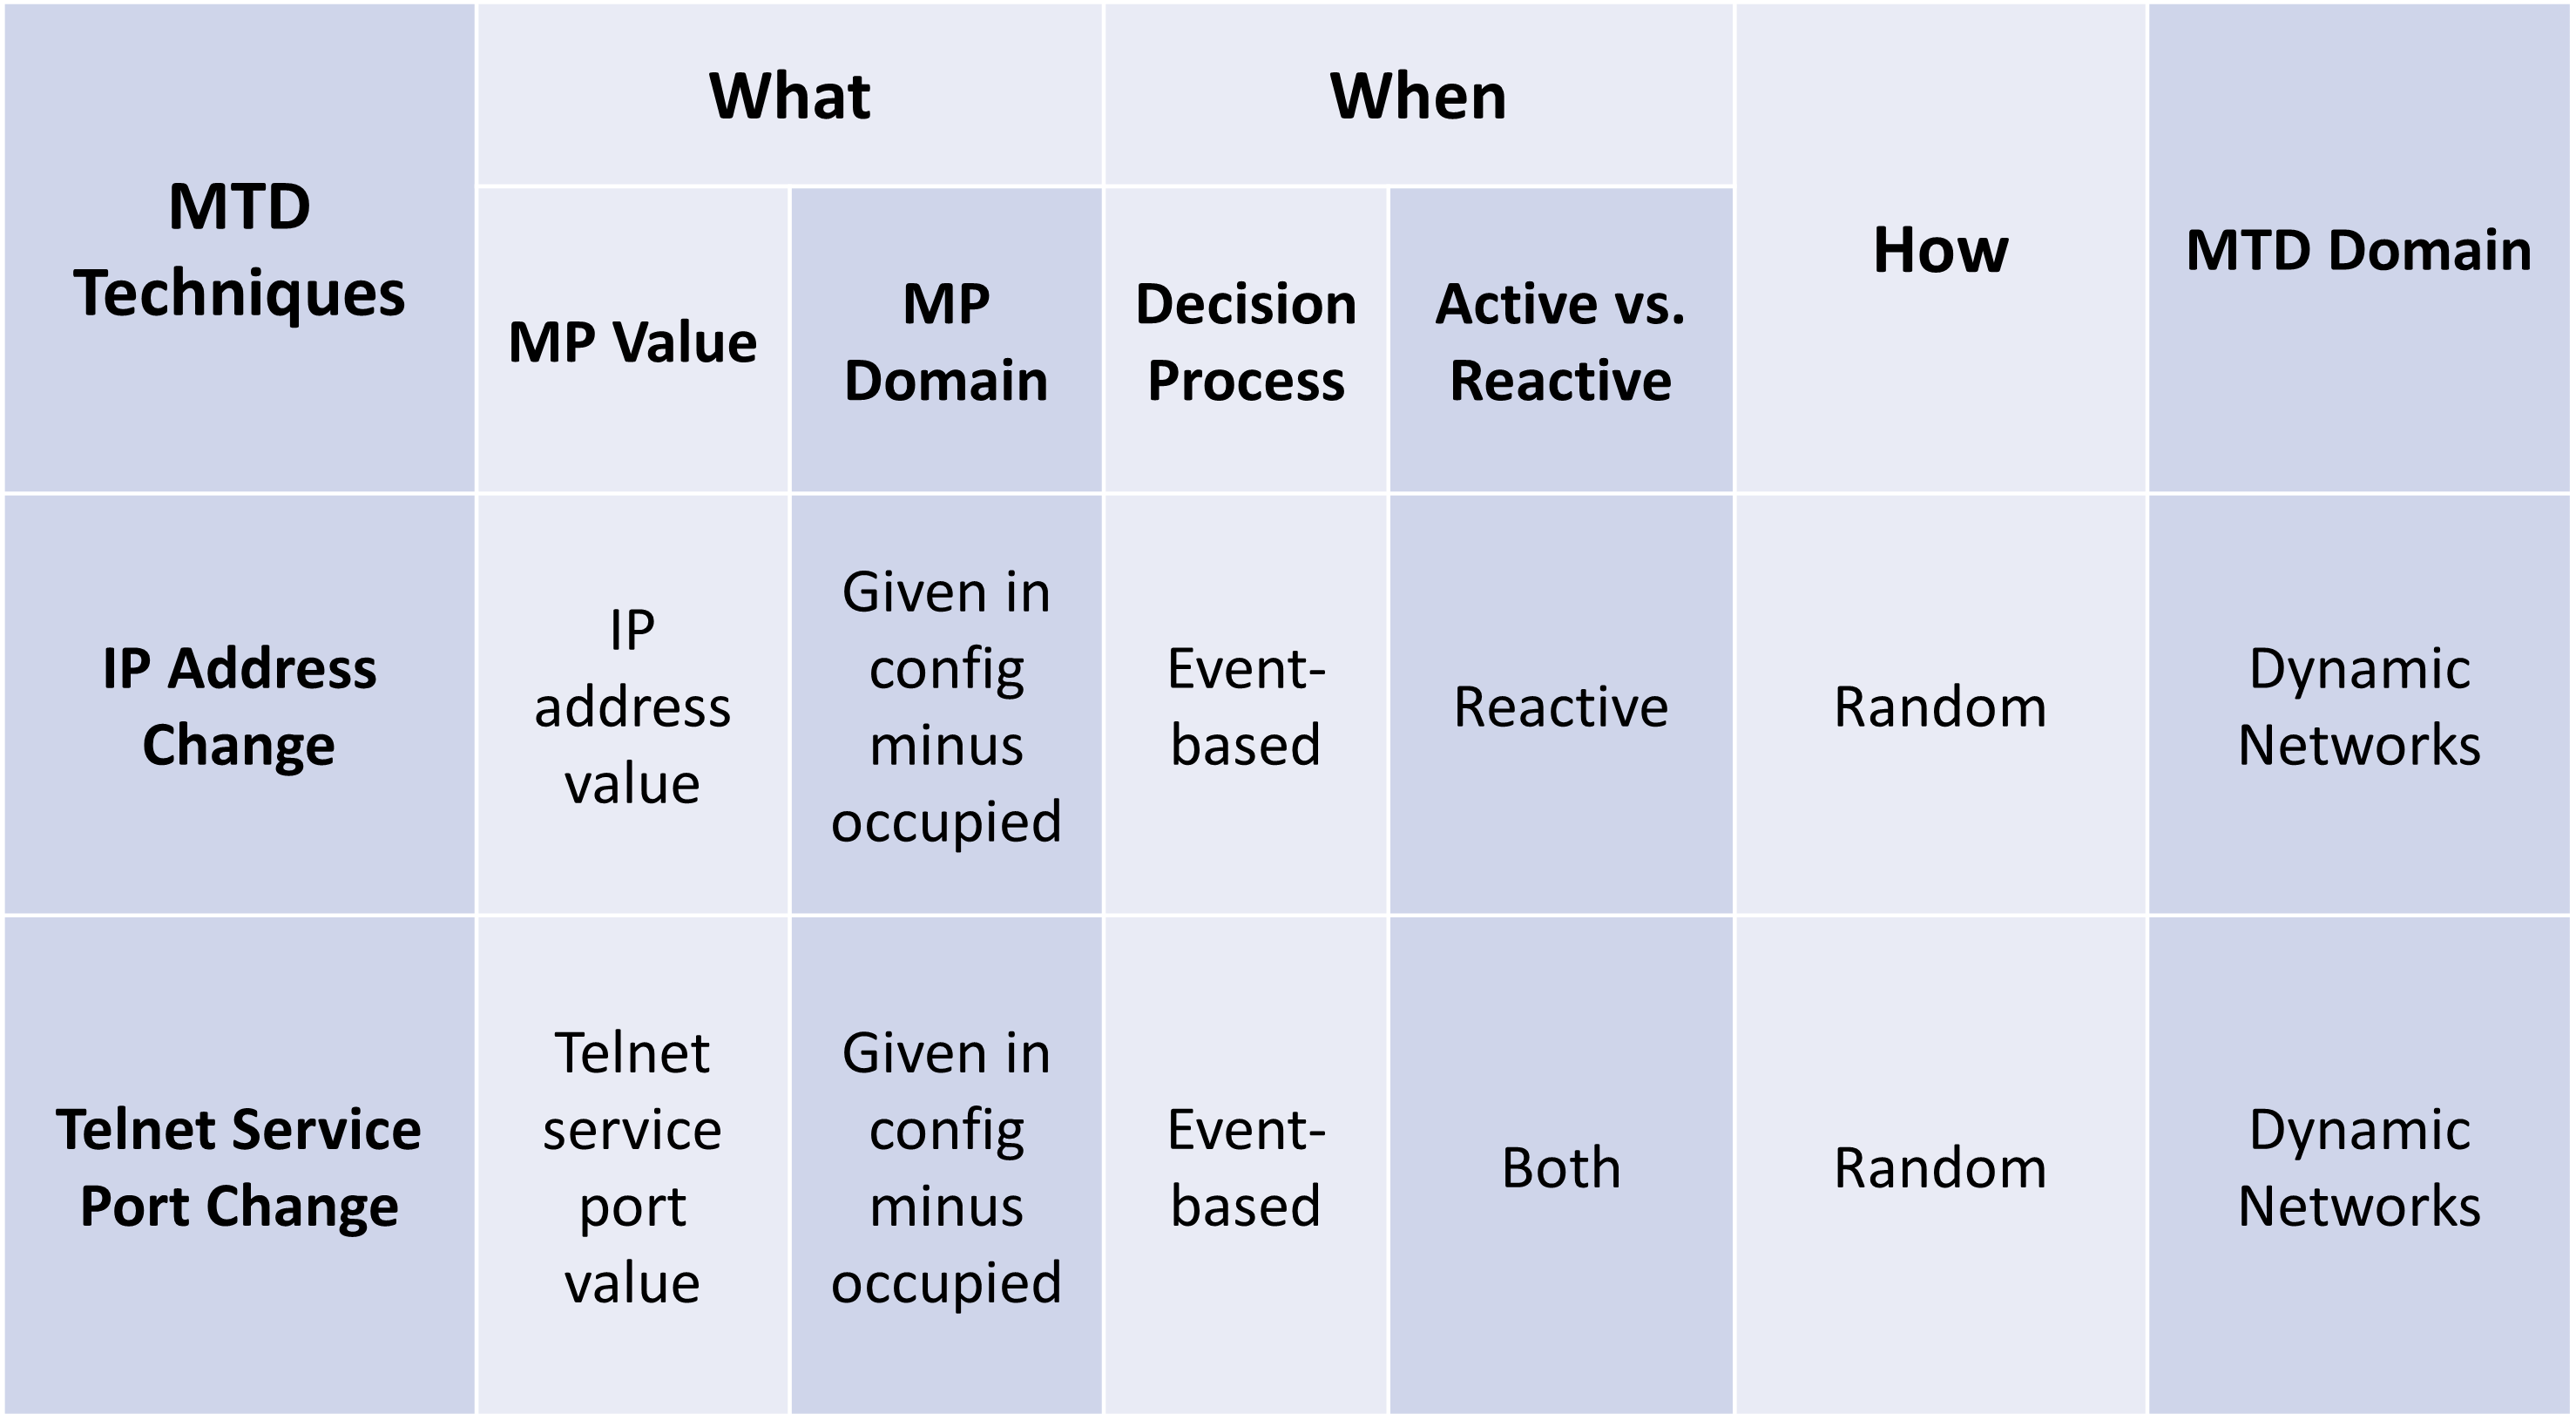
\includegraphics[scale=0.7]{assets/tableAppliedMTDTechniques.png}
\centering
\caption{A Summary of the MTD Techniques Applied With Respect to the Three Fundamental Elements of IoT Techniques.}
    \label{graphic:tableAppliedMTDTechniques}
\end{table}



Although both MTD techniques clearly fall into the dynamic network category, the classification of the attack phase they seek to disrupt is not as straightforward as~\cite{article:okhraviFindingFocus} indicated. The reason for this is that I consider the five-phase attack of~\cite{article:okhraviFindingFocus} to be more applicable when an attacker has a specific target to attack. Bashlite aims to infect as many generic devices as possible, rather than targeting a specific device. However, Bashlite also has its different phases, as shown in Section \ref{analysisOfBashlite}. This allows a comparison between the attack phases specified by~\cite{article:okhraviFindingFocus} and the phases of Bashlite. The scanning phase of Bashlite corresponds to the Reconnaissance and Access phases, as they both attempt to find a target and gather information about it. There is no Bashlite counterpart to the Development phase, as the malware is obviously already developed. The transfer of the client file to the susceptible machine and its execution corresponds to the Launch phase. Although Bashlite does not install any additional backdoors, the fact that the client is connected to a C\&C server could be mapped to the Persistence phase of~\cite{article:okhraviFindingFocus}. The information just described can be seen in Table \ref{graphic:tableBashliteVSAttackPhases}.

\begin{table}[tph]
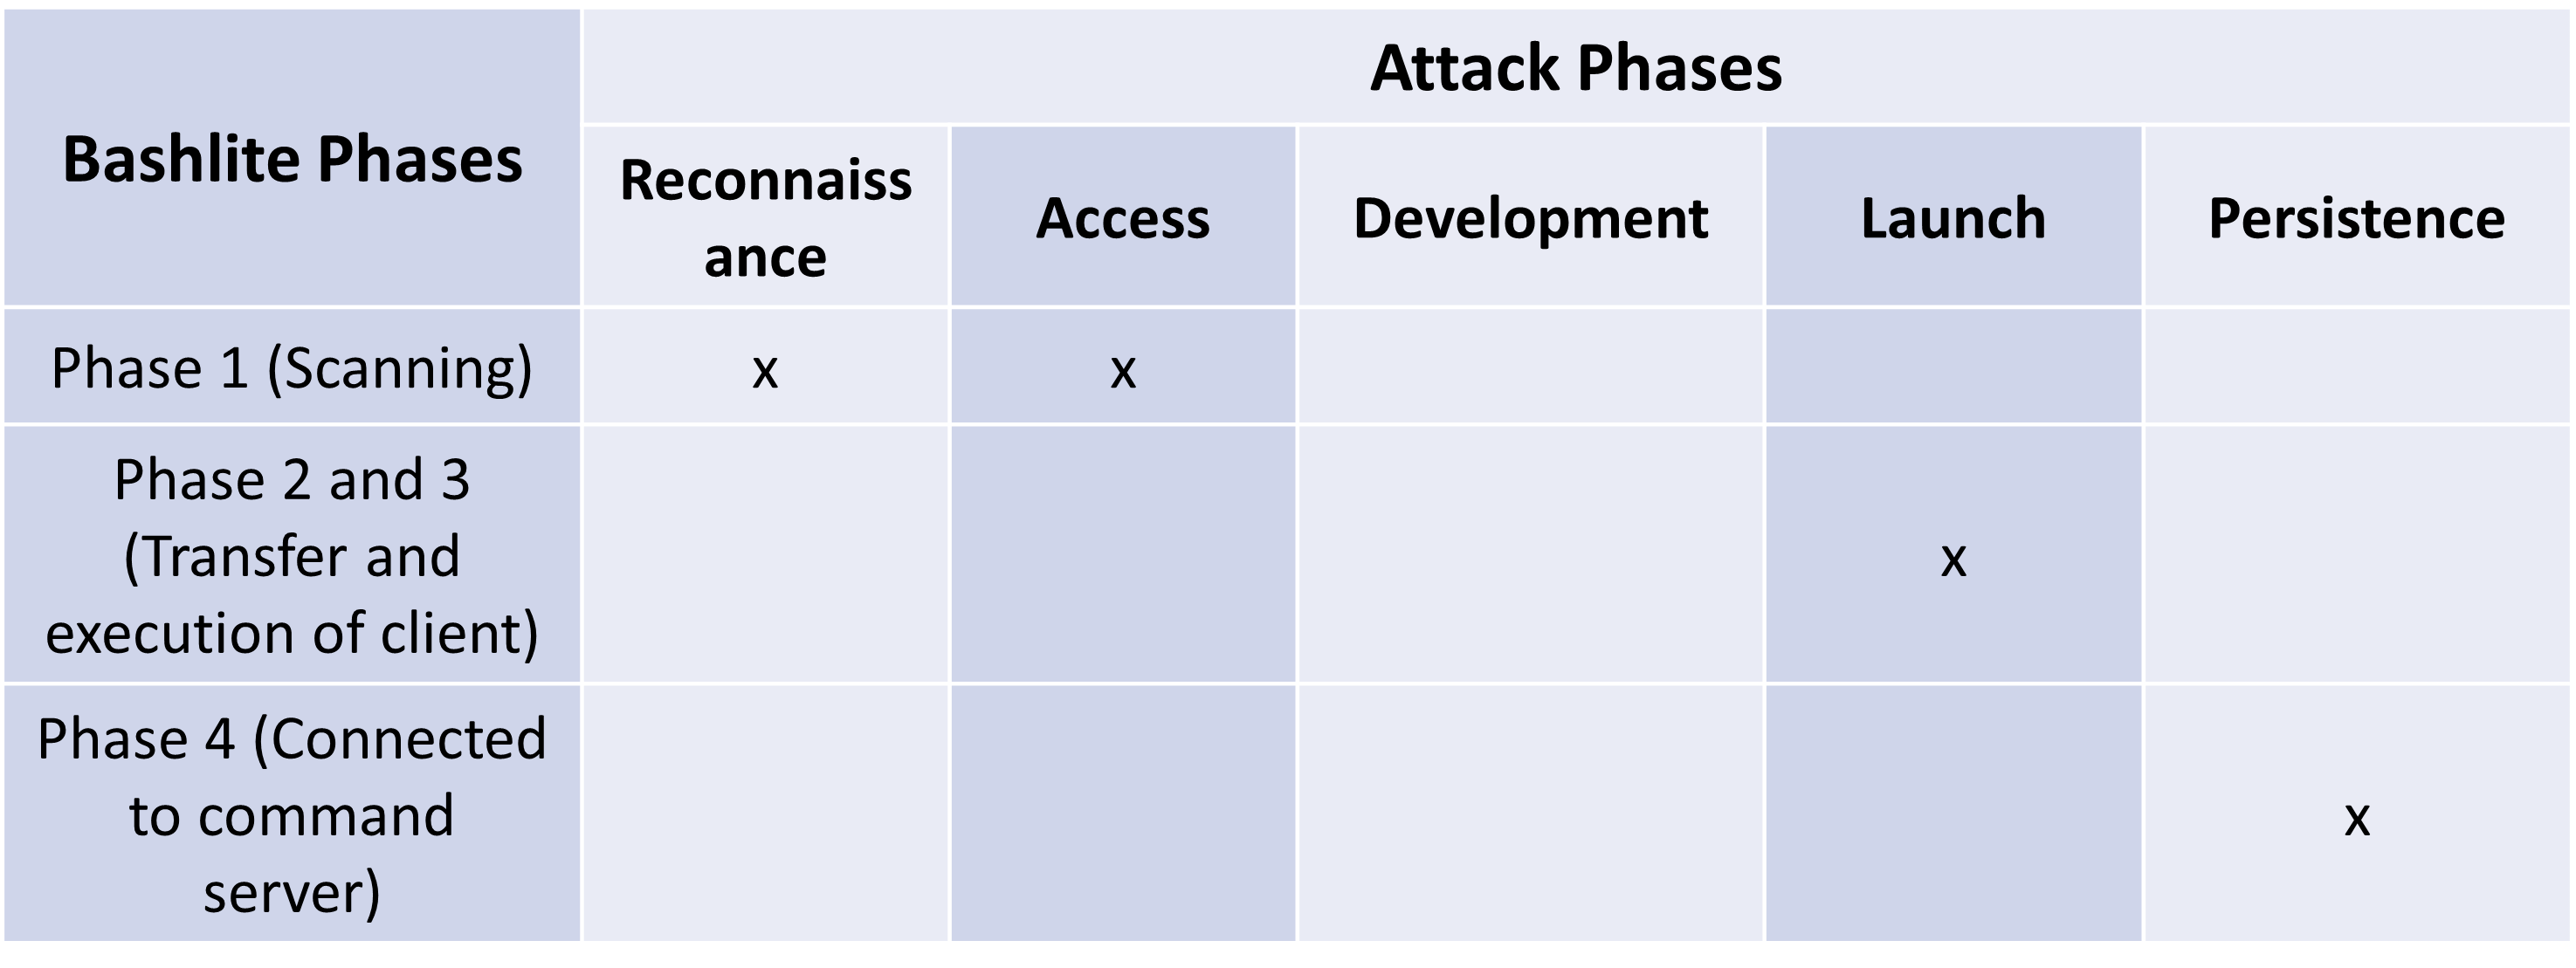
\includegraphics[scale=0.7]{assets/tableBashliteVSAttackPhases.png}
\centering
\caption{The Attack Phases of Bashlite and Their Mapping to the Corresponding Attack Phases.}
\label{graphic:tableBashliteVSAttackPhases}
\end{table}


Since Section \ref{analysisOfBashlite} showed in which phases of Bashlite it is possible to mitigate its infection, this can also be expressed in terms of the attack phases of~\cite{article:okhraviFindingFocus}. Hence, the MTD techniques applied defend against the Reconnaissance phase, the Access phase and the Launch phase.~\cite{article:okhraviFindingFocus} also indicated that Dynamic Network Domain techniques can hinder the Reconnaissance and Launch phases of an attack, but they did not indicate that Dynamic Network Domain techniques can also hinder the Access phase. I assume this is due to the difference in the type of attack (Bashlite vs. specific target).



\subsection{Issues of the Initial Prototype}
\label{section:IssuesOfInitialPrototype}
The first step towards the final implementation was to test whether the initial prototype would still run on the current machines. Unfortunately, this was not the case, as the \textit{ifconfig} command used to change the IP address in the initial prototype in Ubuntu was not suitable for changing the IP address in Raspberry OS. Another problem with the initial implementation was that each machine's IP address was changed. Assuming that a machine is infected and Bashlite starts scanning for other susceptible machines in the LAN, changing the IP address of the other machines would make no difference because Bashlite continues to scan for IP addresses randomly, meaning that another IP address would still be found. 
Furthermore, this thesis has not considered that the LAN setting could have other negative effects. Section \ref{section:futureResearch} briefly discusses this issue, but it was beyond the scope of this thesis to address it.   

%To make this an effective defense strategy for not yet infected devices, we would need to know which IP addresses are already scanned by Bashlite and Bashlite would not be allowed to start scanning again after it finished its scan. Unfortunately, I was not able to test this due to time constraints and my adaptions of Bashlite, but looking at the code of the client, this becomes obvious.  
%Besides of not knowing whether this would be technically feasible, the solution to change the telnet ports is much more convenient and secure. 


%As we have just seen, the IP change alone is not a suitable MTD techniques when dealing with Bashlite. In section \ref{analysisOfBashlite}, I discussed two possible MTD techniques that target the weaknesses of Bashlite and I chose to connect these two. The infected device will change its IP address, the other devices will move the telnet service away from port 23. Like that we can disconnect the infected IP from the command server and at the same time protect all other devices from getting infected. This combination has several advantages based on the type of botnet we look at. As we have seen in section \ref{subsection:P2PIoTBotnets}, P2P IoT botnets are extremely dangerous due to their robustness. My goal was that the solution ideally should protect against classic botnets as well as against P2P IoT botnets. In the following, I will first talk about my implementation and afterwards theoretically analyse how the implementation should work against these two different botnets. 

\subsection{Implementation Details}
This chapter presents and explains the implemented code. It separates the clients, \textit{Deployer Client} and \textit{Deployer Server} as well as possible, but the main goal was to explain the files in the order of the control flow. A recurring Python module in the code is the \textit{subprocess} module for running Bash commands in Python. Two different functions from this module were used, the \textit{subprocess.run()} and the \textit{subprocess.popen()}. A difference between the two is that the \textit{run()} function waits until the Bash command has finished, whereas the \textit{Popen()} executes the command in a child process~\cite{website:pythonSubprocess}. In practice, this means that \textit{subprocess.run()} will cause the Python code to pause its execution until the passed Bash command is complete, and \textit{subprocess.open()} will continue to execute the Python code without waiting for the Bash code to complete. Depending on the Bash command and its goal, it was clear which function was beneficial. 


\subsubsection{Device Sends Information} 
The starting script is \textit{sendToDeployerClient.py}. This script is quite simple and differs significantly from the initial prototype. First it connects to a listening socket created by the \textit{DeployerClient}. This is followed by a try and except block in which the scripts calls a function that starts Bashlite using the \textit{subprocess.Popen()} function. This ensures that Bashlite runs in the background and the Python script can continue. A modified version of Bashlite that immediately starts scanning for susceptible devices saved a lot of time, as there was no need to connect to the server as management and manually start the scanner over and over again. The \textit{sendToDeployerClient.py} script then sleeps for a certain number of seconds. This was to fake the time it took to detect Bashlite, as after this sleep the script sends a "malware found" message to the \textit{Deployer Client} listening socket.



\subsubsection{Deployer Cient Handling Client Information}
The listening socket of the \textit{Deployer Client} is created by the \textit{listenToDevices.py} script. Again, this is a fairly simple script that just listens for virus messages and calls the \textit{send()} function of the \textit{sendToDeployerServer.py} script. This listener supports multiple connections through multithreading. This was necessary because all devices in the LAN should be able to send information to the \textit{Deployer Client} at the same time. In the \textit{send()} function of \textit{sendToDeployerServer.py}, the script connects to the listening socket of the \textit{Deployer Server} and sends another virus message along with the IP address of the infected machine.




\subsubsection{Deployer Server Handling Deployer Client Information}
The \textit{listenToDeployerClient.py} script creates this listening socket and receives the virus message from the \textit{Deployer Client}. This message is then split to filter out the IP address, followed by a call to the main function of the \textit{sendToDevices.py} script with the IP address as an argument. This IP address argument indicates the IP address of the infected device. 

Before explaining the \textit{sendToDevices.py} script, this paragraph briefly explains the \textit{Config.json} file. This is where the user can add configuration values regarding the MTD techniques. The configuration file can be seen in Listing \ref{lst:Config}. There are several key-value pairs for each MTD technique (IP address and Telnet service port change). The rootIP, together with the startIPDevices and endIPDevices, determines the possible range of IP addresses that could be assigned to an infected device. So, in this listing example, the possible IP address of an infected device is in the range between 192.168.1.1 and 192.168.1.90 minus the IP addresses already in use. The server IP is generally used on multiple occasions throughout the code. As for the port change MTD technique, the "startOfPossible" and "endOfPossible" keys define the port range that could replace the Telnet service port on the susceptible devices. The "timeToChangeBack" key specifies the number of seconds that susceptible machines should wait before the Telnet service port is changed back to port 23. This information will eventually need to be sent to the client, but the aim was to have the entire configuration in one place.

\newcounter{temp}
\setcounter{temp}{\value{lstlisting}}
\setcounter{lstlisting}{0}
\renewcommand{\lstlistingname}{Listing}

\begin{lstlisting}[caption={The Configuration File in Which the MTD Values can be Specified.},label={lst:Config}]
{
"IP": {
  "rootIP": "192.168.1",
  "startIPDevices": "1",
  "endIPDevices": "90",
  "serverIP": "10"
  },
"port": {
  "startOfPossible": "3000",
  "endOfPossible": "4000",
  "timeToChangeBack": "300",
}}
\end{lstlisting}

\setcounter{lstlisting}{\value{temp}}
\renewcommand{\lstlistingname}{Algorithm}

The \textit{sendToDevices.py} is one of the two essential files. This file contains two functions. The first is a helper function called \textit{getIPInformation()}. This function takes a set of arguments specified in the Config.json file and returns an IP object containing all the relevant information regarding IP addresses. First, the function creates an array of all possible IP addresses within the range and the server IP address specified in the configuration. Then the function runs a \textit{nmap} scan on that IP range to see which IP addresses are already in use. The function filters the result of the \textit{nmap} with a regex expression, removes the occupied IP addresses from the array of all possible IP addresses, and creates an array in which it puts all occupied IP addresses except the server IP address and the infected IP address. This array is needed later and contains all the IP addresses that may need to move their Telnet service ports for the Telnet service. Finally, the object returned by the \textit{getIPInformation()} function is a dictionary with three key-value pairs containing the IP address of the infected device, the array of all possible/unoccupied IP addresses, and the array of all IP addresses that may need to change their Telnet service ports for the Telnet service.

The other function in the \textit{sendToDevices.py} is the \textit{letExecuteMTDMechanisms()}. This function triggers the start of the MTD techniques on the clients and provides them with the necessary information. It needs the information object returned by the \textit{getIPInformation()} function and other arguments from the configuration file. \textit{letExecuteMTDMechanisms()} starts by assigning the values of the information object to variables to keep the code as clean as possible. This is followed by two main blocks of code, the first dealing with the IP address change of the infected machine and the second dealing with the port change.


The code dealing with the IP address change starts with an if statement to check if an IP address was passed as a parameter in the function call. This allows the user to only change the port if he/she has a use for this, and it allowed to better test the code as it is possible to run the port change MTD technique alone. The if statement is followed by a try and except block to catch any errors. The try block connects to the infected device's listener, picks a random IP address from the array of all possible IP addresses, and sends a message of the form "IP:\textit{IPaddress}". But before this message is sent, a "-1" is sent to the listeners (clients) and the response is received. This was an improvised and slightly unclean fix, but since the client expects one more round of information from the \textit{MTD Deployer Server} in the port change code block than in the IP change code block, this allowed to leave the code as it was on the client side. After the IP message is sent, the port is closed. Again, several exceptions are caught to prevent unexpected code failures. The IP address change code block can be seen in Algorithm \ref{lst:Pseudocode sendToDevicesIP.py}.
\\

\begin{lstlisting}[                
    caption={The Code Block for Changing the IP Address on the Server Side From the \textit{letExecuteMTDMechanisms()} Function in Pseudocode. Everything Related to the Port Change has Been Ommited Here.},label={lst:Pseudocode sendToDevicesIP.py}]
def letExecuteMTDMechanisms(ipInformation,timeToChangeBack,maxTryOfNewPorts,startOfPossiblePorts,endOfPossiblePorts):
    // NOTE: omitted all the code for the port change
    
    SET allPossibleIPS to ipInformation["allPossibleIPs"]
    SET infectedIP to  ipInformation["infectedIP"]
    IF infectedIP is not None:
        TRY:
            CONNECT to client via socket
            SET newIP to random IP of allPossibleIPS
            SEND "-1" to client
            RECEIVE unimportant answer from client
            SEND "IP:newIP" to socket
            CLOSE connection to client
        CATCH ERROR:
            PRINT some kind of error message
    END IF
\end{lstlisting}

The code dealing with the port change starts with a for loop because, unlike the IP address change, the port needs to be changed on multiple devices. So the script iterates through all the IP addresses in the array of IP addresses that might need a port change. This is followed by another try and except block. Several things happen in this try block: a connection is made to the currently iterated IP address, an array is created containing all the ports defined as the port range in the configuration, and a random port is selected to be sent to the device. The script also sends the maximum number of attempts the client should make to migrate to another port. This is followed by two loops to continuously talk to the clients.

The inner while loop continuously sends a message ("port:\textit{Port}") with the randomly selected port to the client, which checks if the port is still available and sends a corresponding response. If the port is available, the script exits the inner loop and continues its execution. If the port is not available on the client, the port is removed from the array of available ports and a new port is randomly selected and sent again. In addition to these two options, the script also handles cases where the maximum number of ports to look up has been reached, or the ports on the client cannot be looked up at all. 

As soon as the code breaks out of the inner loop, the script does nothing, but waits for another message to be received. Here it checks three different cases: either the migration to the new port worked, an error was received, or the client asks for the time after which it should move the telnet service back to port 23. In the first two cases the script returns from the function, in the third case it sends the value of the \textit{timeToChangeBack} key from the configuration file. In the except block, the script catches a \textit{ConnectionRefusedError}, because if a device that should change the port of the Telnet service does not have the listener running, the code would otherwise throw an error and break. The code block for changing the port on the server side can be seen in Algorithm \ref{lst:Pseudocode sendToDevicesPort.py}.
\\

\begin{lstlisting}[caption={The Code Block for Changing the Port of the Telnet Service on the Server Side From the \textit{letExecuteMTDMechanisms()} Function in Pseudocode. Everything Related to the IP Address Change has Been Ommited Here.},label={lst:Pseudocode sendToDevicesPort.py}]
def executeMTDMechanisms(ipInformation,timeToChangeBack,maxTryOfNewPorts,startOfPossiblePorts,endOfPossiblePorts):
    // NOTE: omitted all the code for the IP change
    
    SET IPsToChangePort to ipInformation["IPsToChangePort"]
    FOR each IP in IPsToChangePort:
        TRY:
            CONNECT to IP of client via socket
            SET allPossiblePorts to range in config file
            SET newPort to random port of allPossiblePorts
            SEND maxTryOfNewPorts given in configuration file
            RECEIVE unimporTant answer from client
            SET success to False
            WHILE True:
                WHILE success is False:
                    SEND "PORT:newPort" to socket
                    RECEIVE answer from client:
                    IF answer is that port is free on client:
                        SET success to True
                    ELSE IF answer is that telnet port not retrievable:
                        PRINT some kind of error message
                        CLOSE connection to client 
                    ELSE IF answer is that max attempts are exceeded:
                        PRINT some kind of error message
                        CLOSE connection to client 
                    ELSE:
                        REMOVE newPort from allPossiblePorts
                        SET newPort to random port of allPossiblePorts
                    ENDIF
                END WHILE 
                SET answer to received data from client
                IF answer is that client finished:
                    PRINT success message
                    CLOSE connection to client
                ELSE IF answer is that error ocurred:
                    PRINT some kind of error message
                    CLOSE connection to client
                ELSE IF answer is that client needs num of seconds:
                    SEND seconds to move back from configuration
                ENDIF       
            END WHILE
        CATCH ERROR:
            PRINT some kind of error message
    END FOR
\end{lstlisting}

\subsubsection{Client Handling Deployer Server Information}
The \textit{listenToDeployerServer.py} is the most important script of the whole solution, as it actually executes the MTD techniques on the clients. This is the only script that needs to be run with \textit{sudo}, as some of the Bash commands included require this security privilege. 
The script has four small helper functions and one large helper function. The four small functions include one that writes to a log file called "output.txt", one that queries the current port of the Telnet service on the machine, one that checks if the Telnet service is listening on port 23, and one that kills a potential Telnet process. The logging functionality was crucial for debugging reasons. It helped to detect errors more quickly, and it is also essential in a real-world deployment of the MTD techniques. 
\\

The second little helper function was to query the current port of the Telnet service. This was needed because the change back to port 23 was not implemented from the start. This prevented the need to manually reset to port 23 after each run during the implementation process. More importantly, the Telnet service port query also catches possible errors that might occur in general. The \textit{getTelnetPort()} function first executes the Bash command shown in Algorithm \ref{lst:findTelnet}.

 \begin{lstlisting}[caption={The Bash Command Used to Query the Telnet Service Port.},label= {lst:findTelnet}]
ss -tlpHn | grep inetutils-inetd
\end{lstlisting}

The \textit{ss} command in Algorithm \ref{lst:findTelnet} can be used to examine sockets, similar to netstat~\cite{website:ss}. The options passed are: include tcp sockets, include listening sockets only, include processes, output information without the header, and try not to resolve service names~\cite{website:ss}. Additionally, the code filters with \textit{grep} for "inetutils-inetd", which was used as an identifier for the Telnet process. \textit{Inetd} is a program that listens on certain Internet sockets and decides which program should respond to the request~\cite{website:inet}. Using this as an identifier works perfectly on the VMs because Telnet is the only service on the VMs that uses \textit{inetutils-inetd}. As this may be different on other devices, it is possible that this Telnet port query may fail. To ensure that the script does not query the wrong port for the Telnet service and therefore misbehaves, the script also queries the Telnet service port from the \textit{/etc/services} file and compares the two. If they are identical, all is good, otherwise the script throws an \textit{AttributeError}. The reason for the \textit{AttributeError} is that it is needed anyway in case "ss -tlnpH | grep inetutils-inetd" returns nothing, which would lead to an \textit{AttributeError} caused by the regex the script uses to filter the port.

The third small but important helper function is the \textit{checkIfTelnetWorks()} function. This uses a socket to check if the Telnet service port allows a connection or not. This function is used to check if moving the Telnet service port was successful or not.

The fourth helper function is \textit{killTelnetProcess()}, which does exactly what it says, again using the \textit{subprocess.run()} function to execute the Bash command. The Bash command passed is a \textit{pkill} with an echo, which echoes either "True" or "False" depending on whether \textit{pkill} was successful or not, and logs accordingly.  


 The fifth and larger helper function is the most complex and is called \textit{changePort()}. It again starts with a command passed as an argument to the \textit{subprocess.run()} function. The command can be seen in Algorithm \ref{lst:replaceAndApply}.
 \\
 
 \begin{lstlisting}[caption={The Bash Commands to Replace the old Telnet Service Port With the new one and Apply the Change.},label={lst:replaceAndApply}]
sed -i 's/\<{0}\>/{1}/g' /etc/services
sudo systemctl restart inetutils-inet.service

\end{lstlisting}


The \{0\} and \{1\} in Algorithm \ref{lst:replaceAndApply} are placeholders which are inserted using Python's \textit{string.format()} function. The first line looks for the old Telnet service port number plus "/tcp" (e.g. 23/tcp) in \textit{/etc/services} and replaces it with the new port number plus "/tcp" (e.g. 2255/tcp). Initially, the mistake was made of not looking for the exact string, which led to other ports containing parts of the old port (e.g. 5523/tcp) being changed (e.g. to 552255/tcp). The solution was to surround the first placeholder with "<" and ">", which resulted in an exact search for the value to replace~\cite{website:sed}.

The second line of Algorithm \ref{lst:replaceAndApply} restarts the \textit{inetutils-inet} service, which applies the changes in the \textit{/etc/services} file without rebooting the system. The script then uses the \textit{grep} command to check if the new port can be found in \textit{/etc/services} and echoes accordingly. Depending on the echo, the script logs an error, returns from the function, or continues with the code. Next, the script uses the \textit{checkIfTelnetWorks()} function to see if the Telnet service is still listening on port 23. If it is, the script writes an error to the log file and sends an error message back to the \textit{Deployer Server}. Otherwise, the code logs that the Telnet service is no longer listening on port 23 and sends a "done" to the \textit{Deployer Server}. Additionally, the script triggers the Telnet service to change back to port 23 after a certain number of seconds. This number is also specified in the \textit{Deployer Server} configuration file. 
To initiate this change back, the script uses the \textit{subprocess.Popen()} function instead of the \textit{subprocess.run()} function, as the Python script should continue to run. The command passed as an argument to \textit{subprocess.Popen()} can be seen in Algorithm \ref{lst:backToPort23}.
\\

 \begin{lstlisting}[caption={The Bash Commands to Change Back to the Telnet Service Port 23 Afer a Given Number of Seconds},label={lst:backToPort23}]
printf "$(date +%F\ %H-%M-%S) SHELL: Sleeping for {0} seconds\n" >> output.txt
sleep {0}
sed -i 's/\<{1}\>/23\/tcp/g' /etc/services
sudo systemctl restart inetutils-inetd.service
sleep 7
sudo lsof -i:23 && found="true"
if [ "$found" = "true" ]
then
    printf "$(date +%F\ %H-%M-%S) SHELL: Went from port {2} back to port 23\n\n\n" >> output.txt
else
    printf "$(date +%F\ %H-%M-%S) SHELL: ERROR: The change back to port 23 failed somehow\n\n\n." >> output.txt
fi       
\end{lstlisting}

The first two lines of Algorithm \ref{lst:backToPort23} write a log to the same file where the Python code is logged. Then the script sleeps for the specified number of seconds. Again, these numbers are inserted using Python's \textit{string.format()} function. Lines 4 and 5 are almost identical to the \textit{changePort()} function, except that the target port is now port 23 again. After modifying the \textit{/etc/services} file, the \textit{inetutils-inted.service} is restarted to take effect without rebooting the machine. The script then pauses for 7 seconds to allow the changes to the port to take full effect before continuing. On line 7, the script runs a \textit{lsof} command to check if port 23 is listening again. This is the Bash replacement for the \textit{checkIfTelnetWorks()} function in Python. Ideally the script would check directly with Telnet if the connection is possible, but it was not possible to make this work with the \textit{subprocess} module. If port 23 is listening, the script logs a success message to the log file (on lines 8 and 9), otherwise it logs an error to the log file (on lines 10 and 11). 


The main function of the \textit{listenToDeployerServer.py} script is \textit{listenToDeployer()}. First the listening socket is created, followed by the first while loop. In this loop, the script receives the maximum number of attempts to look for a free Telnet port sent by the \textit{Deployer Server}, which queries the configuration file for the maximum number of attempts. The script then sends a response that the maximum attempts have been received, which also ensures that the \textit{Deployer Server} does not continue with its code as it is forced to wait for a response. A second loop follows in which the script receives another message from the \textit{Deployer Server} that is either "IP:\textit{IPaddress}" or "port:\textit{Port}". This message is split into two variables called "movingParameter" and "movingParameterValue". The script then checks whether the moving parameter is "IP" or " port".

In the IP case, the script closes the listening socket properly, as it would have been closed anyway after the IP change, and all the necessary information has been received. It then kills the Bashlite process. Although the IP change disconnects the Bashlite client from the command server, rendering it harmless, the Bashlite client continues to run on the infected machine, which was tedious for testing. Therefore, the Bashlite client was killed. The IP address of the device is then changed using the command shown in Algorithm \ref{lst:replaceApplyIP}.
\\

\begin{lstlisting}[caption={The Bash Commands to Change the IP Address.},label={lst:replaceApplyIP}]
sed -i 's/\<{0}\>/{1}/g' /etc/dhcpcd.conf
ifconfig eth0 down && sudo ifconfig eth0 up
                
\end{lstlisting}


The first line of Algorithm \ref{lst:replaceApplyIP} replaces the old IP address with the new one in the \textit{etc/dhcpcd.conf} file. The script again inserts the values in Python with the \textit{string.format()} function, therefore the \{0\} and \{1\} in the Bash code. The second line shuts down the Ethernet adapter and restarts it immediately. The Raspberry OS needs to do this to migrate to the new IP address, otherwise the changes would not take effect until the system is rebooted, which is not applicable. After the IP address is changed, the script sleeps for 7 seconds because the Ethernet adapter needs about 5 seconds to reboot. After this time, the script uses the \textit{socket.gethostbyname()} function to get the current IP address of the device, checks whether the IP address change worked or not, and logs a corresponding message. The Python code block for changing the IP address on the clients can be seen in Algorithm \ref{lst:Pseudocode listenToDeployerServerIP.py}
\\

\begin{lstlisting}[caption={The Code Block for Changing the IP Address of a Client From the \textit{listenToDeployer()} Function in Pseudocode. Everything Related to the Port Change of the Telnet Service has Been Ommited Here.},label={lst:Pseudocode listenToDeployerServerIP.py}]
def listenToDeployer(HOST, PORT):
    CREATE listening socket
    WHILE True:
        RECEIVE max attempts for trying to find port (-1 here)
        SEND unimportant answer
        WHILE True:
            RECEIVE command from server
            SPLIT command to movingParameter and movingParameterValue
            IF movingparamter is "IP":
                CLOSE connection to client
                KILL telnet process
                CHECK if telnet process was killed
                CHANGE the IP address
                SLEEP for 7 seconds
                CHECK if the IP change worked
            // NOTE: omitted all the code for the port change
            ELSE
                CLOSE socket
                RETURN
            ENDIF
            
\end{lstlisting}

If the moving parameter is the port, then another machine in the network is infected and the current machine should move its Telnet service port. There is an additional condition in the port case if statement. This condition is whether a count variable is below the maximum number of port change attempts.

The port change code block is more complex than the IP change block above. In a first step, the script checks the \textit{/etc/services} file to see if the random port sent by the \textit{Deployer Server} is free on this device. If the port is found in the services file, the script sends a "taken" message to the \textit{Deployer Server}, which then sends a new random port as described above. If this port is free on the device, the script will query the current Telnet port using the \textit{getTelnetPort()} function described above. The script also calls the \textit{killTelnetProcess()} function. This is necessary because, as mentioned above, if the Bashlite server has already started a connection to this susceptible machine, changing the port of the Telnet service would have no effect, and the Bashlite client would normally start on the susceptible machine. 

Note that the \textit{killTelnetProcess()} function only affects existing connections, not an open Telnet service in general. Nevertheless, the function is called anyway, as there is no downside to calling it. The script then uses the \textit{checkIfTelnetWorks()} function described above to check if the current Telnet service is running on the machine on port 23 or not. If not, the script returns from the \textit{listenToDeployer()} function and logs accordingly, as no measurements are required. Otherwise, the port change is initiated by another function called \textit{changePort()}, which is described in more detail above. This function changes the port of the Telnet service from 23 to another random port sent by the \textit{Deployer Server}, checks if this port change worked, and also changes the Telnet service back to port 23 after a given number of seconds. After this function finished, the socket is closed and the script returns from the \textit{listenToDeployer()} function. The code block for changing the port of the Telnet service on the clients can be seen in Algorithm \ref{lst:Pseudocode listenToDeployerServerPort.py}.
\\





\begin{lstlisting}[caption={The Code Block for Changing the Port of the Telnet Service of a Client From the \textit{listenToDeployer()} Function in Pseudocode. Everything Related to the IP Address Change has Been Ommited Here.},label={lst:Pseudocode listenToDeployerServerPort.py}]
def listenToDeployer(HOST, PORT ):
    CREATE listening socket
    WHILE True:
        SET count to 0
        RECEIVE max attempt for trying to find port
        SEND unimportant answer
        WHILE True:
            RECEIVE command from server
            SPLIT command to movingParameter and movingParameterValue
            IF movingparamter is "IP":
                // NOTE: omitted the code for the IP address change
            ELSE IF movingParameter is port and count <= max attempt:
                INCREMENT count
                CHECK if movingParameterValue (port) is used
                IF port is used:
                    SEND that port is already used
                    CONTINUE with WHILE loop
                ELSE
                    CALL function to get telnet port
                    IF not possible:
                        SEND error
                        CLOSE socket
                        RETURN
                    END IF
                    SEND that port is unused
                    CALL function to kill existing telnet processes
                    CALL function to check if telnet listens on port 23
                    SEND message to get the time to change back
                    RECEIVE time to change back
                    CALL function to change port
                    CLOSE socket
                    RETURN
            ELSE
                SEND max attempt are exceeded
                CLOSE socket
                RETURN
            ENDIF
            
\end{lstlisting}





% bis do ane de text korrigiert und mit writefull drüber








\begin{comment}
\subsection{Things that I could have done differently}
rite bashlite such that it checks for open ports in the lan 

%\subsection{Potential Problems} \label{section:potentialProblems}
When we consider the LAN setting, Bashlite could also theoretically scan for IP addresses in the network as well as all possible ports for this IP devices. I did not create such a Bashlite version, but I   
theoretisch wärs chillimarili zum im bashlite client checke zum d'ip vom host gwechslet het und denn eifach neu zum command server verbinde


\todo{remove the deployer client, it is basically useless and just an additional poit of faiulre and a  similartiy to jordan}
\end{comment}